\documentclass[11pt,reqno]{amsart}

\usepackage{amssymb,mathrsfs,color}
\usepackage{pinlabel}
\usepackage{graphicx}
\usepackage{graphics} 
\usepackage{algorithm}
\usepackage{algorithmic}
\usepackage{natbib}
\usepackage{caption}
\usepackage{tikz}
\usepackage{xspace}


\usetikzlibrary{patterns}


\graphicspath{ {c:/users/mcytrynbaum/documents/rfigures/} {c:/users/mcytrynbaum/Desktop/package/} }
\DeclareGraphicsExtensions{.pdf,.png,.jpg}

\usepackage{amsmath} % for all math functions and operations
\usepackage{amsfonts} % use this to write scripts (e.g. Real nums, etc)
\usepackage{mathtools} %for other math stuff not included in packages above
\usepackage{amsthm} % in case you want the THM: COR: LEMMA: setup
\usepackage[top=1in,bottom=1in,left=1in,right=1in]{geometry} %for setting the margins

%\setlength\parindent{0pt}

\newtheorem{thm}{Theorem}[section]
\newtheorem{lemma}[thm]{Lemma}
\newtheorem{prop}[thm]{Proposition}
\newtheorem{cor}[thm]{Corollary}
\newtheorem{subroutine}[thm]{Subroutine}
\theoremstyle{definition}
\newtheorem{defn}[thm]{Definition}
\newtheorem{examp}[thm]{Example}
\newtheorem{remark}[thm]{Remark}
\setcounter{equation}{0}
\numberwithin{equation}{section}

\renewcommand{\algorithmicrequire}{\textbf{Input:}}
\renewcommand{\algorithmicensure}{\textbf{Output:}}
\newcommand{\prf}{\begin{proof}}
\newcommand{\eprf}{\end{proof}}
\newcommand{\lft}{\left(}
\newcommand{\rt}{\right)}
\newcommand{\be}{\beta}
\newcommand{\eps}{\epsilon}
\newcommand{\wh}{\widehat}
\newcommand{\wt}{\widetilde}
\newcommand{\al}{\alpha}
\newcommand{\bp}{\begin{pmatrix}}
\newcommand{\ep}{\end{pmatrix}}
\newcommand{\inv}{^{-1}}
\newcommand{\var}{\text{Var}}
\newcommand{\cov}{\text{Cov}}
\newcommand{\corr}{\text{Corr}}
\newcommand{\ssumi}{\sum_{i=1}^n}
\newcommand{\ssumj}{\sum_{j=1}^n}
\newcommand{\ssumk}{\sum_{k=1}^n}
\newcommand{\im}{\text{Im}}
\newcommand{\mc}{\mathcal}
\newcommand{\mr}{\mathbb{R}}
\newcommand{\ol}{\overline}
\newcommand{\ul}{\underline}
\newcommand{\prob}{\mathbb{P}}
\newcommand{\ital}{\emph}
\newcommand{\tb}{\textbf}
\newcommand{\pa}{\partial}
\newcommand{\et}{\eta}
\newcommand{\argmax}{\operatornamewithlimits{argmax}}
\newcommand{\lag}{\langle}
\newcommand{\rag}{\rangle}

\newcommand{\pre}{\phi}
\newcommand{\econ}{e}
\newcommand{\coordpre}{\mathrm{CP}}
\newcommand{\prealloc}{(2^X)^A}
\newcommand{\sub}{\subseteq}
\newcommand{\strcore}{\mathrm{C}(X,U)}
\newcommand{\core}{\mathrm{WC}(X,U)}
\newcommand{\stable}{\mathrm{S}(X,U)}
\newcommand{\fecon}{\mathrm{E}}
\newcommand{\fix}{\mathcal{E}}
\newcommand{\suq}{\succeq}
\newcommand{\peq}{\preceq}
\newcommand{\su}{\succ}
\newcommand{\pe}{\prec}
\newcommand{\toppre}{\ol{\pre}}
\newcommand{\bopre}{\ul{\pre}}
\newcommand{\strongc}{\mathcal{G}}
\newcommand{\strongcomp}{S}
\newcommand{\acto}{Q_0} 
\newcommand{\actok}{Q_0^k} 
\newcommand{\actokk}{Q_0^{k+1}} 
\newcommand{\actot}{Q_0^t} 
\newcommand{\actott}{Q_0^{t+1}} 
\newcommand{\actol}{Q_0^{\ell}} 
\newcommand{\actoll}{Q_0^{\ell + 1}} 
\newcommand{\acta}{Q_A} 
\newcommand{\actak}{Q_A^k} 
\newcommand{\actakk}{Q_A^{k + 1}} 
\newcommand{\actc}{Q_I} 
\newcommand{\actck}{Q_I^k} 
\newcommand{\actckk}{Q_I^{k + 1}} 
\newcommand{\actat}{Q_A^t} 
\newcommand{\actatt}{Q_A^{t + 1}} 
\newcommand{\actct}{Q_I^t} 
\newcommand{\actctt}{Q_I^{t + 1}} 
\newcommand{\act}{Q} 
\newcommand{\actt}{Q_{temp}} 
\newcommand{\actacum}{\wh{Q_A}} 
\newcommand{\actocum}{\wh{Q_0}} 
\newcommand{\disto}{d}
\newcommand{\distt}{D}
\newcommand{\preo}{\pre^{0}} 
\newcommand{\pren}{\pre_{0}} 
\newcommand{\pref}{\pre^{f}} 
\newcommand{\coll}{I}
\newcommand{\collk}{I^k}
\newcommand{\res}{\act_{int}}
\newcommand{\reach}{H}
\newcommand{\forest}{F}
\newcommand{\fixfind}{\mathcal{E}_C}
\newcommand{\fixfindk}{\mathcal{E}^k_C}
\newcommand{\fixfindkk}{\mathcal{E}^{k + 1}_C}
\newcommand{\fixtemp}{\mathcal{E}_{temp}}
\newcommand{\fixtempk}{\mathcal{E}^k_{temp}}
\newcommand{\fixtempkk}{\mathcal{E}^{k + 1}_{temp}}
\newcommand{\fixtempt}{\mathcal{E}^t_{temp}}
\newcommand{\fixtemptt}{\mathcal{E}^{t + 1}_{temp}}
\newcommand{\stp}{\mathrm{STOP}}
\newcommand{\pair}{(F,I)}
\newcommand{\roott}{R}
\newcommand{\depth}{D}
\newcommand{\unproc}{\mathcal{J}_u}
\newcommand{\glob}{G}
\newcommand{\optwo}{T_2}
\newcommand{\opthree}{T_3}
\newcommand{\oper}{F}
\newcommand{\point}{P}
\newcommand{\lattice}{L}

\newcommand{\topx}{\ol{X}}
\newcommand{\topy}{\ol{Y}}
\newcommand{\botx}{\ul{X}}
\newcommand{\boty}{\ul{Y}}
\newcommand{\pairi}{(X_i,Y_i)}
\newcommand{\pairj}{(X_j,Y_j)}
\newcommand{\pairp}{(X',Y')}
\newcommand{\pairpp}{(X'',Y'')}

%%%% ALGORITHM CONTROLS
\newcommand{\infcombiniti}{(i)\xspace}
\newcommand{\infcombinitii}{(ii)\xspace}
\newcommand{\infcombinitiii}{(iii)\xspace}
\newcommand{\infcombgraphi}{(1)\xspace}
\newcommand{\infcombgraphii}{(2)\xspace}
\newcommand{\infcombgraphiii}{(3)\xspace}
\newcommand{\infcombcomba}{(a)\xspace}
\newcommand{\infcombcombb}{(b)\xspace}

\newcommand{\infacredi}{(i)\xspace}
\newcommand{\infacredii}{(ii)\xspace}
\newcommand{\infacbstopa}{(a)\xspace}
\newcommand{\infacbstopb}{(b)\xspace}
\newcommand{\infacstoptwi}{(i)\xspace}
\newcommand{\infacstoptwii}{(ii)\xspace}
\newcommand{\infacstoptwiii}{(iii)\xspace}
\newcommand{\infacstoptha}{(a)\xspace}
\newcommand{\infacstopthb}{(b)\xspace}
%%%%

\date{Novemeber 21, 2015}
\title{Using Lattice Geometry to Find All Stable Allocations}
\author{Max Cytrynbaum} 
\thanks{I am very grateful to Scott Kominers for continual guidance and for providing the inspiration for this project. This project was completed with the help of an Economic Design Summer Fellowship from the Harvard Society of Fellows. Please send comments and suggestions to mcytrynbaum@gmail.com.}

\begin{document}
\maketitle
\begin{abstract}
In this paper, we give an algorithm to find all core allocations in a highly general model of multilateral many-to-many matching with contracts.
We develop a notion of information sharing in lattices, showing how lattice geometry and information sharing can be exploited to produce a relatively fast algorithm that returns the full list of core outcomes.
We show how to apply this technique to more general economic problems and, as an application, construct the first algorithm to find \emph{all} stable allocations in bilateral matching with contracts and substitutable preferences. 
\end{abstract}

\section{Introduction}
\subsection{Introduction and Motivation}
This paper extends an algorithm pioneered in \cite{EcheniqueYenmez2013} to find \emph{all} core allocations in a general model of multilateral many-to-many matching with contracts.
Our model nests a large number of previously considered matching models.
We show that, as in the case of matching with preferences over colleagues in \cite{EcheniqueYenmez2013}, core allocations can be characterized in terms of the fixed points of an antitone operator on a certain complete lattice.
Our main contribution is to show how to fully exploit the geometric relationships implied by the problem's lattice structure.
We develop a notion of information sharing in lattices, construct and prove correctness for an algorithm that implements this idea, and show how this approach may be extended to a wider class of economic problems for which there is a complete lattice structure. 
To conclude, we restrict our attention to two-sided many-to-many matching with contracts with substitutable preferences, showing how information sharing may be used to find \emph{all} stable allocations.

There are a variety of results showing the existence of a lattice of stable outcomes when preferences satisfy a substitutability condition.
Usually, these results proceed by showing that substitutability implies the existence of an isotone operator on a complete lattice containing the stable matchings\footnote{See, for instance, \cite{HatfieldMilgrom2005} or \cite{HatfieldKominers2010}.}.
By iteration from a maximal element, one eventually arrives at an extremal stable matching.
Conversely, in the absence of substitutability, not only are stable matchings not guaranteed to exist, but the usual isotone operator is not guaranteed to find any that do exist.
Even if substitutability does hold, it is often unclear how to find any but the extremal stable matchings.

This paper aims to address some of these issues.
The core is a natural replacement for stability in the absence of substitutability guarantees; indeed, in many classical models, such as the marriage problem, the core coincides with the set of stable matchings\footnote{\cite{RothSotomayor1990}.}. 
We show that, even without a substitutability guarantee, in which case the usual operator for finding stable matchings is not necessarily isotone, there still exists a relatively fast algorithm that returns all \emph{core} allocations or shows that none exist. 
When substitutability does hold, we show how our technique can be modified to find \emph{all} stable matchings, not just the extremal ones.

As noted by \cite{KlausKlijn2005}, substitutability is an unreastically stringent condition in many real world markets.
Thus, our algorithm has practical value for a market designer interested in finding reasonable economic outcomes in such markets.

Lattice structures arise frequently in economics.
We show how lattice geometry can be combined with economic problem structure to develop a notion of information sharing in lattices that allows for faster computation of objects of economic interest.  
The algorithm developed in this paper thus has independent economic value outside of matching theory. 

\subsection{Related Literature}

This paper is related to a broad literature on finding stable outcomes.
\cite{RothPeranson1999} is a well-known computational study examining the existence of stable outcomes in the National Residency Matching Program. 
For classical matching problems, \cite{Martinezetal2004} develops an algorithm for finding all stable matchings in a many-to-many matching market, while \cite{McvitieWilson1971} and \cite{IrvingLeather1986} show how to find all stable matchings in one-to-one matching markets.
More recently, papers such as \cite{Sethuramanetal2006} and \cite{SchwarzYenmez2011} have shown how to find ``median'' stable matchings, which in some sense balance the interest of market participants. 
See \cite{GusfieldIrving1989} for a review of algorithms for finding all core matchings in the classical setting.

The algorithm developed in this paper is an extension of antitone operator approach developed in \cite{Echenique2007Equilibria} and \cite{EcheniqueYenmez2013}.
\cite{kominers2010matching} shows that this approach finds all stable matchings in classical matching, while \cite{Kojima2007b} shows how to extend the approach to the case of matching with couples.


\section{Characterizing Core Allocations} \label{section:strcore}
In this section, we show how core allocations can be characterized as the fixed points of an antitone operator on a certain complete lattice.
First, we give details on our model and notation.

\subsection{Model and Solution Concepts}
We consider a finite set of contracts $X$, each of which is associated with at least one agent $a\in A$. 
We call a subset $Y\sub X$ an \emph{allocation}, and let $2^X$ denote the set of all allocations. 
Let $d(x)$ be the set agents associated with a contract $x\in X$, and extend this definition to allocations by writing $d(Y) \equiv \bigcup_{y\in Y} d(y)$.
Note that, in general, we may have $|d(x)| > 2$ for multilateral contracts.
For instance, we can view $X$ as the set of potential multilateral relationships in a trading network\footnote{This setting is thus a slight generalization of \cite{HatfieldKominers2010} model of bilateral contracts in a trading network.}. 
In particular, we \emph{do not} impose a two-sided market structure in this section.

For $a\in A$, we let $Y_a = \{y\in Y: \, a\in d(y)\}$ denote the set of contracts associated with that agent (note that we may have $Y_a = \emptyset$). Thus, $2^{X_a}$ denotes the set of all allocations naming an agent $a\in A$. 
We assume that each $a\in A$ has strict preferences over $Y \in 2^{X_a}$, where the utility of an allocation is given by the one-to-one function $U_a: 2^{X_a} \to \mr$.
Let $\su_a$ denote the strict preference relation induced by these utility functions over bundles $Y \in 2^{X_a}$, with $\suq_a$ denoting the weak relation. Thus, $Y \suq_a  Z \iff$ $Y \su_a Z$ or $Y = Z$.
Throughout this paper, we will assume that $\emptyset_a \in X$ for all $a \in A$, where $\emptyset_a$ denotes $a$ being unmatched. Note that $d(\emptyset_a) = \{a\}$. 

An allocation $Y \sub X$ is said to be in the \emph{core}\footnote{The core concept defined here is sometimes also called the strong core or ``core by weak domination''; see \cite{RothSotomayor1996}, for instance.
Here, we follow the core concept used in \cite{EcheniqueYenmez2013}.}
if there does not exist a non-empty blocking set $Z \sub X$ such that 
\[
U_b(Z_b) \geq U_b(Y_b) \qquad  \forall b\in d(Z)
\]
where \emph{at least one} of the above inequalities holds strictly.
We denote the core by $\strcore$. 

Similarly, an allocation $Y$ is said to be in the \emph{weak core} if there does not exist a non-empty blocking set $Z \sub X$ such that 
\[
U_b(Z_b) > U_b(Y_b) \qquad  \forall b\in d(Z)
\]
We denote the weak core by $\core$. 
Note that $\core \supseteq \strcore$.

It is easy to see that core allocations need not exist in such a general setting.
Our approach will be to construct an algorithm that either finds all core allocations or shows that none exist. 

\subsection{Fixed Preallocations and the Core}
We build an appropriate framework in which to generalize the fixed point construction discussed above. 
We start by generalizing the classical notion of a \emph{prematching}. 

\begin{defn}[Preallocation] We call a map $\pre: A \to 2^X$ a \emph{preallocation} if $\pre(a) \in 2^{X_a}$ for all $a\in A$. Let $(2^X)^A$ denote the set of all preallocations.  
\end{defn}

Intuitively, a preallocation assigns each agent to a bundle of contracts naming him or her. We may think of $\pre(a)$ as the set of contracts ``held'' by agent $a$.   

We can associate each allocation $Y\subseteq X$ with a unique preallocation $\pre_Y$ in a natural way by setting $\pre_Y(a) = Y_a$ for $a \in d(Y)$ and $\pre_Y(a) = \emptyset_a$ otherwise.
\begin{remark} Note, however, that not all preallocations can be derived from allocations in this way.
For example, consider the case where $\emptyset \not = \pre(a)_b \not = \pre(b)_a$. In the preallocation $\pre$, $a$ holds contracts naming $b$ that are \emph{not} in the bundle of contracts held by $b$ naming $a$.  
In particular, there does not exist an allocation $Y$ such that $\pre = \pre_Y$. 
\end{remark}

With this example in mind, we say that $\pre \in \prealloc$ is a \emph{coordinated} preallocation if there exists an allocation $Y$ such that $\pre = \pre_Y$. 
We denote the set of all cooordinated preallocations by $\coordpre\sub \prealloc$.
Our method proceeds by identifying allocations $Y \in \strcore$ with fixed points of an operator on preallocations, generalizing the construction in \cite{EcheniqueYenmez2013}.

For each agent $a \in A$, we define 

\[
V(\pre, a) = \{Z \in 2^{X_a}: \exists Y \in 2^X \, s.t. \,  Y_a = Z, \, Y_b \suq_b \pre(b) \: \forall b \in d(Y)\setminus\{a\} \}
\]

Intuitively, $V(\pre, a)$ is the \emph{possibility set} for an agent $a$ at a preallocation $\pre$. 
It contains all bundles of contracts naming $a$ that are part of a larger economy $Y$ in which every other agent $b \in d(Y)$ weakly prefers their contracts under $Y$ to their contracts under the preallocation $\pre$.  

Next, we define an operator $T: \prealloc \to \prealloc$ by setting $T \pre(a) = \max V(\pre, a)$, where the maximum is taken under the preference relation $\suq_a$ for each $a \in A$.
Note that $\emptyset_a \in V(\pre,a)$ for any $\pre \in \prealloc$, so $T$ is well-defined. Let $\fix(T)$ denote the fixed points of $T$. Define $\fecon(T) = \{Y \in 2^X: \, \pre_Y \in \fix(T)\}$, the collection of allocations $Y$ whose corresponding preallocation $\pre_Y$ is fixed by $T$.

Before our first result, we note a simple fact: if $\pre \in \coordpre$, then $\pre(a) \in V(\pre, a)$.
To see this, note that $\pre \in \coordpre$ means that there exists $Y \sub X$ with $\pre = \pre_Y$. 
Then $Y$ is an allocation satisfying the conditions in $V(\pre_Y,a)$, so that $Y_a  = \pre(a) \in V(\pre,a)$. 
With the definitions above, we have a simple result
\begin{lemma} \label{lemma:strictcore}
$\fecon(T) = \strcore$
\end{lemma}
\prf
First, suppose that $Y \not \in \strcore$. Then by definition, there exists some blocking allocation $\emptyset \not = Z \sub X$ such $Z_b \suq_b Y_b$ for all $b \in d(Z)$.
Let $a \in d(Z)$ be such that the inequality above is strict, and consider $\pre = \pre_Y$. 
In particular, $Z_b \suq_b \pre_Y(b)$ for all $b \in d(Z) \setminus \{a\}$, so that $Z_a \in V(\pre_Y, a)$.
Then $T \pre_Y(a) = \max V(\pre_Y, a) \suq_a Z_a \su_a Y_a = \pre_Y(a)$, so $T\pre_Y(a) \not = \pre_Y(a)$, and $Y \not \in \fecon(T)$.  

Suppose, conversely, that $Y \not \in \fecon(T)$ so that $\pre_Y \not \in \fix(T)$.  
Then there exists an agent $a \in A$ such that $T\pre_Y(a) = Z_a \not = \pre_Y(a)$ for some allocation $Z$.  
By the definition of $V(\pre_Y,a)$, we have $Z_b \suq_b \pre_Y(b) = Y_b$ for $b \in d(Z) \setminus \{a\}$.
We know $\pre_Y$ is coordinated, so by the simple fact above $\pre_Y(a) \in V(\pre_Y,a)$.
Then $Z_a = T \pre_Y(a) \su_a \pre_Y(a) =  Y_a$. Then $Z$ is a blocking coalition for $Y$, so $Y \not \in \strcore$.  
\eprf
Thus, we have identified $\strcore$ with the set of \emph{coordinated} preallocations $\pre \in \coordpre$ such that $T \pre = \pre$. 
This result shows that an algorithm that finds all $\pre \in \fix(T)$ will also find all core matchings. 

However, if there are \emph{uncoordinated} preallocations that are also fixed by $T$, such an algorithm may return extraneous solutions not associated with any core matching.
The following lemma, which is essential for the construction of our algorithm, shows that there are no such preallocations.
Note that this result significantly generalizes the corresponding lemma in \cite{EcheniqueYenmez2013} and also subsumes the main result of \cite{Kojima2007b}. 

\begin{lemma} \label{lemma:coordinated}
$\fix(T) \sub \coordpre$
\end{lemma}
\prf
We begin with an important fact that will be used repeatedly.
Suppose that $\pre \in \fix(T)$. Then for any $a \in A$, we have $\pre(a) = T\pre(a) \in V(\pre,a)$.
Thus, there exists an allocation $Y$ such that $Y_a = \pre(a)$, and $Y_b \suq_b \pre(b)$ for all $b \in d(Y) \setminus \{a\}$.
Since $Y_a = \pre(a)$, then in fact $Y_b \suq_b \pre(b)$ holds \emph{for all} agents $b \in d(Y)$. 
For any $b \in d(Y)$, $Y$ then satisfies the conditions in the definition of $V(\pre,b)$, so $Y_b \in V(\pre,b)$. 
Therefore, $\pre(b) = T\pre(b) \suq Y_b \suq \pre(b)$, so equality holds throughout. In particular, $Y_b = \pre(b)$ for all $b \in d(Y)$. 

Fix $a_1 \in A$. Since $\pre \in \fix(T)$, the argument above shows that there exists an allocation $Y$ such that $Y_{a_1} = \pre(a_1)$, and, in particular, $Y_b = \pre(b)$ for all $b \in d(Y)$. 
Therefore, the collection of global allocations available to $a_1$ at $\pre$ 
\[\glob(\pre,a_1) = \{Y \in 2^X: Y_{a_1} = \pre(a_1), \: Y_b \suq \pre(b)\: \forall b \in d(Y)\}\]
is non-empty, so there exists an allocation 

\[
Y \in \argmax_{Z \in \glob(\pre,a_1)} |d(Z)|
\]

Let $A_1 = d(Y)$. If $A_1 = A$, we are done, since then by the construction above $Y_a = \pre(a)$ for all $a \in A$, so $\pre = \pre_Y$ and $\pre \in \coordpre$. 

Then assume that $A_1 \not = A$, and pick $a_2 \in A \setminus A_1$. By the fact at the beginning of the proof, there exists an allocation $Z$ such that $Z_{a_2} = \pre(a_2)$, and, in fact, $\pre(b) = Z_b$ for all $b \in d(Z)$. 
Define $A_2 = d(Z) \cap A_1^c$, which is non-empty by construction.
Let $b \in A_2$. We will show that $d(\pre(b)) \cap A_1 = \emptyset$.
That is, under the preallocation $\pre$, agent $b \in A_2$ is \emph{not} holding any contracts that name agents in $A_1$. 

Suppose not, so there exists $c \in A_1 \cap d(\pre(b))$.
Then, in particular, $c \in d(\pre(b)) = d(Z_b) \sub d(Z)$, so applying the fact proved at the beginning, $Z_c = \pre(c) = Y_c$. 
Since $c \in d(Z_b)$, there exists a contract $z \in Z_c$ naming both $c$ and $b$.
Then $b \in Z_c = Y_c$, so $b \in d(Y_c) \sub d(Y) = A_1$, so $b \in A_1 \cap A_2 = \emptyset$. 
This is a contradiction, so it must be the case that $d(\pre(b)) \cap A_1 = \emptyset$ for all $b \in A_2$. 

Define $S = \bigcup_{b \in A_2} \pre(b)$. We have just shown that $d(S) \sub A_1^c$.
We also have $d(S) = \bigcup_{b \in A_2} d(\pre(b)) = \bigcup_{b \in A_2} d(Z_b) \sub d(Z)$, so $d(S) \sub A_1^c \cap d(Z) = A_2$.
Clearly $b \in d(\pre(b))$ for all $b \in A_2$, so $A_2 \sub d(S)$. Then $A_2 = d(S)$. 

Set $W = Y \cup S$. We have now shown that $A_2 \not = \emptyset$ and $A_1 \cap A_2 = \emptyset$.
Since $d(Y) = A_1$ and $d(W) = A_2$, it follows that $W \cap Y = \emptyset$, so we have  

\begin{enumerate}
\item $W_b = Y_b = \pre(b)$ for all $b \in A_1$.
\item $W_b = S_b = \pre(b)$ for all $b \in A_2$.
\end{enumerate}

Then apparently $W \in \glob(\pre,a_1)$ as defined above. However, by construction $|d(W)| > |d(Y)|$, which contradicts our original choice of $Y$.
This finishes the proof.
\eprf
\subsubsection{Discussion}
Combining these lemmas, we see that searching for core allocations in a very general model of multilateral matching with contracts is equivalent to searching for the fixed points of $T$. 
Our algorithm depends heavily on this result, which shows, critically, that the fixed points $\fix(T)$ are only as dense in $\prealloc$ as the core outcomes.

Our maximal domain results will show that this is not the case for the natural extension of this method to \emph{weak} core outcomes $\core$.
For weak core outcomes, where the lattice algorithm fails, $T$ also fixes at a large number of extraneous, uncoordinated preallocations (see Lemma~\ref{lemma:core}). 

\subsection{The Lattice of Fixed Preallocations}
In this section, we generalize constructions from \cite{EcheniqueYenmez2013} showing the the fixed points of the squared operator $T^2$ form a lattice. 
First, we define a natural partial order on the set of preallocations $\prealloc$.

Say that $\pre \su \pre'$ if and only if $\pre(a) \suq_a \pre'(a)$ for all $a \in A$, where at least one of these inequalities \emph{holds strictly}. 
Thus, we write $\pre \suq \pre'$ if and only if $\pre \su \pre'$ or $\pre = \pre'$. 
This is a product order on a product space, which makes $\prealloc$ into a complete lattice. 
Next, we give a sequence of results concerning the operator $T$ and its fixed points. 
These results are an almost direct extension of the results in Lemma 4 through Proposition 8 of \cite{EcheniqueYenmez2013}.
For the purposes of illustration, we include the proof the first result for the more general framework of preallocations considered in this paper.
The rest of the lemmas follow from straightforward extensions of the work in \cite{EcheniqueYenmez2013}. 
\begin{lemma} \label{lemma:antitone}
$T$ is antitone 
\end{lemma}
\prf
Let $\pre \peq \pre'$ be preallocations.
Fix $a \in A$, and let $Z \in V(\pre',a)$.
Then there is an allocation $Y \sub X$ with $Y_a = Z$ such that $Y_b \suq_b \pre'(b)$ for $b \in d(Y) \setminus \{a\}$.
Then $Y_b \suq_b \pre'(b) \suq_b \pre_b$ also for all such agents, so we also have $Z \in V(\pre,a)$.
Then $V(\pre,a) \supseteq V(\pre',a)$, so that $T\pre(a) \suq T\pre'(a)$. The agent $a$ was arbitrary, so $T\pre \suq T\pre'$ under our partial order. 
\eprf
The following lemmas follow exactly as in \cite{EcheniqueYenmez2013}, using the antitonicity of $T$. 
\begin{cor} $T^2$ is isotone, and $\fix(T^2)$ is a non-empty complete lattice. 
\end{cor}
\begin{lemma} \label{lemma:order}
No two preallocations $\pre$ and $\pre'$ can be compared under the partial order on $\prealloc$.
\end{lemma}
\begin{lemma} \label{lemma:top}
There exist preallocations $\ol{\pre}$ and $\ul{\pre}$ such that for all $\pre \in \fix(T)$, we have $\ol{\pre} \suq \pre \suq \ul{\pre}$. Moreover, if $\pre = \ol{\pre}$ or $\pre = \ul{\pre}$, then $\fix(T) = \{\pre\}$. 
\end{lemma}

\section{Sharing Lattice Information to Find All Core Allocations}
\subsection{Introduction}
In this section, we give an algorithm that finds \emph{all} core allocations in the model of multilateral matching with contracts considered above.
Our algorithm builds upon the original approach in \cite{EcheniqueYenmez2013}.
In particular, we show how to fully exploit the problem's complete lattice structure to more efficiently find the full set of core matchings. 

The algorithm proceeds by successively initializing modified versions of the original matching problem, in which each agent has a truncated preference list.
Our main contribution is to realize that many of the subproblems created while searching the lattice $\fix(T^2)$ share geometric information with other subproblems.
We show how fast digraph algorithms may be used to combine this shared information and more quickly identify the full set of core matchings. 

\subsection{Intuition and Notation} \label{section:description1}
\subsubsection{Algorithm Intuition}
Let $\pre^*$ denote the largest preallocation under the partial order $\su$.
That is, $\pre^*(a) = \argmax U_a(\pre(a))$ for each $a \in A$.
Suppose that the total number of agents $|A| = m > 0$.
We will use $\langle \pre \rangle$ or $\langle \pre(1) \hdots \pre(m) \rangle$  to denote a version of the original problem in which each agent $a$'s preference list is truncated to allocations in $2^{X_a}$ ranked weakly below $\pre(a)$ by agent $a$. 
We will often identify a problem $\lag \pre \rag$ with its maximal point $\pre$.
Let $\fix(\pre) \equiv \{\pre' \in \fix(T): \: \pre' \peq \pre\}$ denote the fixed points of $T$ below $\pre$.  

By Tarski's Theorem\footnote{This is easy to see.
Note that $T^2 \pre^* \peq \pre^*$ by maximality, so $(T^2)^k \pre^* \peq (T^2)^{k+1} \pre^*$ for any $k\geq 1$ by isotonicity.
Then this sequence is monotonically decreasing and bounded above $\min \fix(T^2)$ on a finite lattice, so it converges in finitely many iterations, say at $k = \ell$.
Let $\pre' \in \fix(T^2)$ another fixed point, then $\pre^* \suq \pre'$, so $\toppre = (T^2)^{\ell} \pre^* \suq (T^2)^{\ell} \pre' = \pre'$, so $\toppre = \max(\fix(T^2))$.}, the sequence $(T^2)^k \pre^*$ converges to a preallocation $\toppre$, fixed by $T^2$, which is the maximal point of the lattice $\fix(T^2)$.
If $T \toppre = \toppre$, then by Lemma~\ref{lemma:top} showing that no elements of $\fix(T^2)$ are ranked by ``$\peq$'', $\fix(T) = \{\toppre\}$.
So suppose that $T \toppre \not = \toppre$. 
Clearly $\fix(T) \sub \fix(T^2)$ for any operator, and, by iteratively applying $T^2$, we have learned that $\fix(T) \sub \fix (T^2) \sub \{\pre': \pre' \peq \toppre\} \equiv \{\pre' \peq \toppre\}$.
We will sometimes denote relations of this type by $\fix(T) \peq \toppre$. 

Since $T\toppre \not = \toppre$, apparently $\fix(T) \sub \bigcup_{i = 1}^m \{\pre' \peq \toppre - e_i\}$, where $e_i$ denotes the standard unit vector\footnote{identifying $\prealloc$ with a grid in $\mr^m$ as above.} in $\mr^m$. 
Consider a subproblem of the form $\lag \toppre - e_i \rag$, and let $T_i$ be the operator corresponding to this subproblem, where agents' preferences are truncated above $\toppre - e_i$.
The key insight of \cite{Echenique2007Equilibria}, which generalizes to the current model, is that $\fix(T) \cap \{\pre' \leq \toppre - e_i\} \sub \fix(T_i)$.
That is, the fixed points of $T$ contained in the cone $\{\pre' \peq \toppre - e_i\}$ are also fixed points of the new problem $\lag \toppre - e_i \rag$ with operator $T_i$. 
Then apparently we have $\fix(T) \cap \{\pre' \leq \toppre - e_i\} \sub \fix(T_i) \sub \fix(T_i^2)$, so information about the lattice of fixed points of $T_i^2$ can be used to bound $\fix(T)$.
The general result in our setting is as follows 
\begin{lemma} \label{lemma:contain}
Suppose $\pre \peq \wh{\pre}$, and let $\wh{T}$ denote the core operator for the problem $\lag \wh{\pre} \rag$.
If $\pre \in \fix(T)$, then $\pre \in \fix(\wh{T})$.
In particular, $\fix(T) \cap \{\pre \leq \wh{\pre}\} \sub \fix(\wh{T}^2)$. 
\end{lemma}
\prf
Let $\wh{V}(\pre, a)$ be the defining set for $\wh{T}$ in the subproblem.
Then for any $a \in A$ and $\pre \in \prealloc$ we have 
$\wh{V}(\pre,a)  = \{Z \in 2^{X_a}: \exists Y \in 2^X \, s.t. \,  Y_a = Z, \, \wh{\pre}(b) \suq_b Y_b \suq_b \pre(b) \: \forall b \in d(Y)\setminus\{a\} \}$
then clearly $\wh{V}(\pre,a) \sub V(\pre,a)$.  
We can compute $\wh{T}\pre(a) = \max \wh{V}(\pre,a) \leq \max V(\pre,a) = T\pre(a)$ for any preallocation $\pre$. 

Now, suppose that $\pre \in \fix(T)\cap\{\pre' \peq \wh{\pre}\}$.
Then we have have $\pre(a) = T\pre(a) \suq_a \wh{T}\pre(a)$ for all $a \in A$. 
By Lemma~\ref{lemma:coordinated} above, $\fix(T) \sub \coordpre$, so $\pre = \pre_Y$ for some allocation $Y \in 2^X$.
In particular, $Y_a = \pre(a) \peq_a \wh{\pre}(a)$, so $\pre(a) \in \wh{V}(\pre,a)$.
Then by the definition of $\wh{T}$, we get $\wh{T}\pre(a) \suq_a \pre(a)$. 

Combining this with the statement above, we have $\pre(a) = \wh{T} \pre(a)$, so $\pre \in \fix(\wh{T})$. 
\eprf 
Returning to the discussion above, we showed that $\fix(T) \sub \bigcup_{i = 1}^m \{\pre' \peq \toppre - e_i\}$, a union of cones in the lattice of preallocations. 
That is, $\fix(T) \sub \bigcup_{i = 1}^m \fix(\toppre - e_i)$.
Fix $i$ and consider $\fix(\toppre - e_i)$, the fixed points of $T$ below $\toppre - e_i$.
For convenience, denote $S_i \equiv T_i^2$ and $\toppre_i \equiv \toppre - e_i$.
Starting with $\toppre_i$, the unanimously most preferred preallocation in the subproblem $\lag \toppre_i \rag$, Lemma~\ref{lemma:strictcore} and the Tarski argument used above show that each iteration of $S_i$ gives a ``cone guarantee'' on the fixed points $\fix(T)$ of the form $\fix(\toppre_i) \peq S_i^k \toppre_i$.

Pursuing this strategy for $i = 1 \hdots m$, we can bound the complete set of fixed points $\fix(T)$ in a union of subproblem cones. 
We continue this strategy recursively by generating $m$ new subproblems whenever a monotonic sequence of the form $S_i^k \toppre_i $ stops at a fixed point of $S_i^k$. 
In this way, we will eventually find the full set of core outcomes, directly extending the \cite{EcheniqueYenmez2013} algorithm to the present setting.  

However, depending on the structure of the lattice $\fix(T^2)$, the strategy described above can actually be quite similar to greedy search.  
In particular, the number of subproblems generated at the kth recursive level scales exponentially in $k$ as $|A|^k$.As we will show, many of the subproblems generated by this strategy are either redundant or do not need to be solved completely.
We will show that we can capitalize on the structure of the preallocation lattice by allowing subproblems to share geometric information with each other. 
With this modification, evaluation of the full Tarski sequence $S_i^k \toppre_i$ is often unnecessary. 
In fact, it is often the case that subproblems can be stopped or removed entirely after a few iterations. 
We will illustrate this idea with a couple of simple examples.  

\subsubsection{Graph-Theoretic Notation}
First, we briefly recall some graph-theoretic notation, which will be useful in the coming sections. A \emph{graph} is a pair $(V,E)$, where $V$ is a collection of \emph{vertices} and $E \sub V \times V$ is a collection of \emph{edges}.
In a \emph{directed graph} (digraph), the order of vertices in an edge matters. 
A \emph{directed path} is a sequence $e^1 \hdots e^n$ of edges, where $e_2^k = e_1^{k+1}$ for $k \leq n-1$. 
A subset $W \sub V$ is \emph{strongly connected} if for any $v_i, v_j \in W$, there exist directed paths $v_i \to v_j$ and $v_j \to v_i$ using only vertices in $W$. 
Strong connectedness is an equivalence relation on $V$, and the (disjoint) maximal strongly connected subsets of $V$ are called the \emph{strong components} of $G$, which we denote by $\strongc$. 
Weak connectedness is defined similarly for an undirected graph, where an (undirected) path is defined as above, ignoring the order on vertices in an edge. 
The \emph{reachable set} from a vertex $v$ is the set of all $v' \in V$ such that there exists a directed path $v \to v'$.  

By a \emph{rooted tree}, we mean a graph that is connected with no cycles (paths starting and ending at the same vertex) and has one vertex designated as the \emph{root}. 
Edges on a rooted tree are naturally oriented away from the root. 
A collection of such rooted trees is called a \emph{forest} and, for such a collection, for a vertex $w$ we let $r(w)$ denote the root of the tree containing $w$, and we let $c(w)$ denote the \emph{children} of $w$, the vertices connected by an edge to $w$ on a path away from the root, and $p(w)$ denote the parent vertex of $w$, defined similarly\footnote{See, for instance, \cite{GrossYellen2005graph} for a more detailed introduction to graph-theoretic terminology.}.

\subsubsection{Example 1 - Colliding Subproblem Cones}
In this section, we give a simple example of how subproblems can share information.
For easy of visualization, consider the case $|A| = 2$. As noted previously, we may identify $\prealloc$ with a grid, in this case in $\mr^2$.
As above, we iterate $T^2$ to find $\toppre = \max \fix(T^2)$, which we identify, for instance, with the integer lattice point $(10,10) = \toppre$. 
Using the notation above, there are isotone operators $S_1 = T_1^2$ and $S_2 = T_2^2$ corresponding to the subproblems $\lag \toppre - e_1 \rag$ and $\lag \toppre - e_2 \rag$, respectively. 

Beginning with subproblem 1, suppose that $S_1 (9,10) = (8,10)$, $S_1^2 (9,10) = (7,9)$, and $S_1^3 (9,10) = (7,9)$.
By our arguments above, we now have a cone guarantee on the fixed points in the first subproblem; specifically, $\fix(T) \cap \{(x,y) \peq (9,10)\} \peq (7,9) \peq (10,9) = \toppre_2$.
Therefore, $\fix(\toppre_1) = \fix(T) \cap \{(x,y) \peq (9,10)\} \sub \fix(T) \cap \{(x,y) \peq (10,9)\} = \fix(\toppre_2)$. 
That is, the solutions to subproblem 1, the fixed points of $T$ in $\{(x,y) \peq (9,10)\}$, are \emph{contained} in the set of solutions to subproblem 2. 

Now suppose that we stop working on subproblem 1 and begin iterating with $S_2$.
Suppose that $S_2(10,9) = (10,6) = S_2^2(10,9)$, so the sequence stops.
Then we have learned that $\fix(\toppre_1) \sub \fix(\toppre_2) \peq (10,6)$. 
However, by iterating $S_1$, we also learned that $\fix(\toppre_1) \peq (7,9)$. 
Then apparently $\fix(\toppre_1)$ is contained in the cone intersection $\{(x,y) \peq (7,9)\} \cap \{(x,y) \peq (10, 6)\} = \{(x,y) \peq (7,6) \}$. 
That is, by \emph{combining the information} from subproblem 2 with subproblem 1, we have learned that $\fix(\toppre_1) \peq (7,6)$. 

\begin{figure} \label{fig:rectangles}
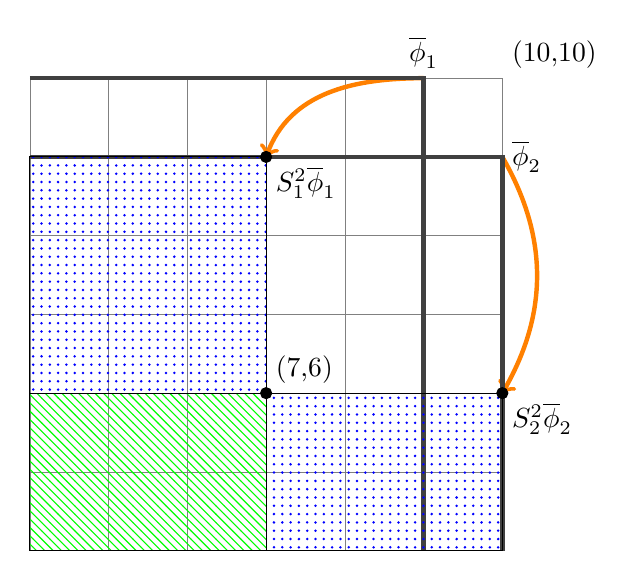
\begin{tikzpicture}
\draw[help lines] (0,0) grid (6,6);
%\draw[fill] (5,6) circle [radius=0.05];
%\draw[fill] (6,5) circle [radius=0.05];
\draw[orange,->, ultra thick] (5,6) to [out=180, in=70] (3,5);
\draw[orange,->, ultra thick, bend left] (6,5) to (6,2);
\draw[darkgray, ultra thick] (0,6) -- (5,6) -- (5,0);
\draw[darkgray, ultra thick] (0,5) -- (6,5) -- (6,0);
\draw[blue] (0,5) -- (3,5) -- (3,0);
\draw[blue] (0,2) -- (6,2) -- (6,0);
\draw[pattern = dots, pattern color = blue] (0,5) rectangle (3,2);
\draw[pattern = dots, pattern color = blue] (3,0) rectangle (6,2);
\draw[pattern = north west lines, pattern color = green] (0,0) rectangle (3,2);
\node[above right] at (6,6) {(10,10)};
\node[above right] at (3,2) {(7,6)};
\node[above] at (5,6) {$\toppre_1$};
\node[right] at (6,5) {$\toppre_2$};
\node[below right] at (3,5) {$S_1^2 \toppre_1$};
\node[below right] at (6,2) {$S_2^2 \toppre_2$};
\draw[fill] (3,2) circle [radius=0.07];
\draw[fill] (3,5) circle [radius=0.07];
\draw[fill] (6,2) circle [radius=0.07];
\end{tikzpicture}
\caption{Combining Information from Subproblem Cones Guarantees}
\end{figure}

Note that, even if we learn $\fix(\toppre_1) \sub \fix(\toppre_2)$, we may still wish to retain the information associated with subproblem 1. 
If, for instance, the outcome for subbproblem 2 was instead that $S_2(10,9) =  (9,6) = S_2^2(10,9)$, then we would also know that $\fix(\toppre_2) \sub \fix(\toppre_1)$, so that $\fix(\toppre_2) \peq \min((9,6),(7,9)) = (7,6)$ and, in fact, $\fix(\toppre_1) = \fix(\toppre_2)$.
The idea of equivalent subproblems is explored further in the next example. 

\subsubsection{Example 2 - Chutes and Ladders}
In this section, we give intuition for how to efficiently combine information and track the relations between different subproblem cones. 
Consider the case $|A| = 3$, where we identify $(10,10,10) = \toppre = \max \fix(T)$. 
After initializing subproblems at $(9,10,10)$, $(10,9,10)$ and $(10,10,9)$, suppose that we find $S_1(9,10,10) = (9,8,10)$, $S_2(10,9,10) = (10,9,7)$, and $S_3(10,10,9) = (9,10,9)$. 
As argued above, this shows that $\fix(\toppre_1) \peq (9,8,10) \peq (10,9,10) = \toppre_2$, so that $\fix(\toppre_1) \sub \fix(\toppre_2)$. 
Similarly, our calculations with $S_2$ and $S_3$ show that $\fix(\toppre_2) \sub \fix(\toppre_3)$ and $\fix(\toppre_3) \sub \fix(\toppre_1)$. 
Combining all these relations, apparently $\fix(\toppre_1) = \fix(\toppre_2) = \fix(\toppre_3) \peq (9,8,7)$, so the subproblems are equivalent.  
Thus, we can collapse all of these subproblems to a new subproblem started at $\pre' = (9,8,7)$ \emph{without losing any fixed points} of the original operator $T$. 

We have seen that collisions between subproblem cones give information relations of the form $\fix(\toppre_i) \sub \fix(\toppre_j)$ regarding the fixed points of $T$.
Consider a digraph that tracks these collisions.
Then this digraph has the form shown below, where subproblems correspond to vertices, and there is an edge $v_i \to v_j$ only if problem $i$ ``collides'' with problem $j$ (made precise below). 
Since, in particular, the digraph has a directed edge $(v_i,v_j)$ only if $\fix(\pre_i) \sub \fix(\pre_j)$, the equivalence of subproblems is reflected in the connectedness of the graph. 

\begin{figure} \label{fig:digraph}
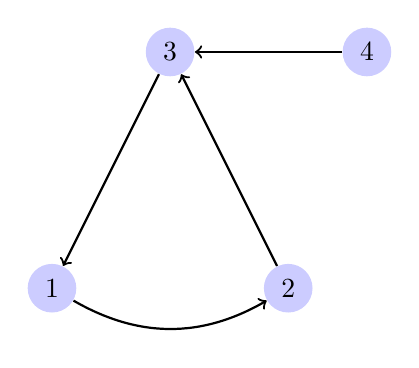
\begin{tikzpicture}

\tikzset{vertex/.style = {circle, fill =blue!20}}
\tikzset{edge/.style = {->, thick}}
%\draw[help lines] (0,0) grid (6,6);
\node[vertex] (a) at (0,1) {1};
\node[vertex] (b) at (3,1){2};
\node[vertex] (c) at (1.5,4){3};
\node[vertex] (d) at (4,4){4};

\draw[edge] (a) to[bend right] (b);
\draw[edge] (b) to (c);
\draw[edge] (c) to (a);
\draw[edge] (d) to (c);
\end{tikzpicture}
\caption{A Collision Digraph}
\end{figure}

Suppose now that $\toppre$ is found at some intermediate step in the algorithm, and consider a distinct subproblem near $\toppre$ started at $\pre_4 = (11,11,11)$ with associated isotone operator $S$.
We begin iterating and find that $S(\pre_4) = (10,10,8)$, which shows $\fix(\pre_4) \sub \fix(\toppre_3)$ 
Then a \emph{single iteration} of $S$ has shown us that $\fix(\pre_4) \sub \fix(\toppre_3) \peq (9,8,7) = \pre'$, using the relations above. 
Of course, the same conclusion would hold if we found that  $S(\pre_4) \peq \toppre_i$ for any $i$. 

We know that $\fix(\toppre_1) = \fix(\toppre_2) = \fix(\toppre_3) \peq \pre'$. 
We can track these subproblem relations efficiently with a collection of rooted trees as follows: let vertices $w_1,w_2,w_3$ be children of $w(\pre')$, a vertex representing $\pre' = (9,8,7)$. 
We denote this relationship by $c(w(\pre')) = \{w_1,w_2,w_3\}$.
Using the notation in the previous section, we have the root-vertex relation $r(w_i) = w(\pre')$ for $i = 1,2,3$. 
Note that, by our work above, we have $\fix(\pre') = \fix(\toppre_i)$ for all $w_i \in c(w(\pre'))$. 
Also, $\fix(\toppre_i) = \fix(\toppre_j)$ for all $i,j$ children of the same node. 

Suppose we maintain a collection of trees for which parent nodes and child nodes are all related in this way. 
Consider a solved subproblem $\lag \pre_i \rag$ with $r(w_i) = w_k$.
Then if at some step of the algorithm we obtain a guarantee that $\fix(\pre_j) \sub \fix(\pre_i)$ for an active subproblem $\lag \pre_j \rag$, the relations built into our problem tree imply that, in fact, $\fix(\pre_j) \sub \fix(\pre_k)$, potentially \emph{skipping a large region of lattice space} that we would otherwise have to search for elements of $\fix(T)$. 
This dynamic gives our algorithm a ``Chutes and Ladders'' effect. 
In particular, we make efficient use of both the geometric information shared between active problems and the information gained during previous steps of the algorithm. 

\begin{figure} \label{fig:forest} 
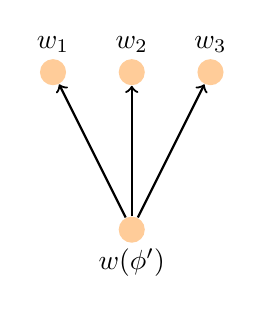
\begin{tikzpicture}
\tikzset{vertex2/.style = {circle, fill =orange!40}}
\tikzset{edge/.style = {->, thick}}

\node[vertex2] (e) at (3,1) {};
\node[vertex2] (f) at (2,3) {};
\node[vertex2] (g) at (3,3) {};
\node[vertex2] (h) at (4,3) {};

\draw[edge] (e) to (f);
\draw[edge] (e) to (g);
\draw[edge] (e) to (h);

\node[above = .12cm] at (f) {$w_1$};
\node[above = .12cm] at (g) {$w_2$};
\node[above = .12cm] at (h) {$w_3$};
\node[below = .12cm] at (e) {$w(\pre')$};

\end{tikzpicture}
\caption{A Problem Forest}
\end{figure}

\subsection{Informal Algorithm Description} 

In this section, we introduce notation and give a brief, intuitive explanation of the full algorithm, building on the examples above.
Pseudocode and correctness proofs for the full algorithm follow. 
First, we discuss indexing. 

\emph{Labels for Preallocations, Vertices, and Operators}:
During the algorithm, we build various graphs.
For any such graph, each vertex will correspond to a problem $\lag \pre \rag$, where $\pre \in \prealloc$.
We thus require a way to denote correspondences between vertices and problems.
We thus fix an index set $\mathcal{I}$, which we use to label problems and vertices.
We will denote corresponding vertices and problems with the same subindex, for instance, $\pre_i \sim v_i \sim w_i$, where $i \in \mathcal{I}$. 
We allow the possibility that $\pre_i = \pre_j$ as preallocations for $i \not = j$.
Thus, technically, a problem $\pre_i$ is a preallocation index pair $(\pre,i) \in \prealloc \times \mathcal{I}$, and we enforce that the index of every problem initialized during the algorithm is chosen to be unique.
When clear, we let $v(\pre)$ and $w(\pre)$ denote the vertices corresponding to a certain problem $\lag \pre \rag$, where $w(\pre) = w_k$ for some $k \in \mathcal{I}$.
Thus, for instance, $v(\pre_i) = v_i$.
For clarity, vertices of a digraph $G$ are always denoted by $v$, while vertices of a forest $F$ are always denoted by $w$.
Similarly, the operator for a subproblem $\pre_i$ will be denoted by $T_i$.
The algorithm consists of two alternating stages. 

\emph{Stage 1 - Information Acquisiton}: In the first stage, we consider a set of problems $\acto$.
As above, each problem $\lag \pre_i \rag$ is associated with an isotone operator $S_i = T_i^2$.
In this stage, we iteratively apply $S_i$ to each $\pre_i \in \acto$, creating new problems when necessary, as discussed below. 
Let $\act$ be a set of problems $\acto \sub \act$, which we think of as the problems from previous steps of the algorithm that still contain useful information.  

\emph{Stopping Conditions}:
During the algorithm, for a problem $\lag \pre_i \rag $, we compute the Tarski sequence $(T_i^2)^k \pre_i$, $k \geq 0$. 
Define the following stopping conditions for an element $ (T_i^2)^k \pre_i \equiv \pre'$ of this sequence.
\begin{enumerate}
\item $\pre' \peq \bopre$ \label{cond:bottom1}
\item $T_i^2 \pre'= \pre'$ \label{cond:fix1}
\item There exists $\pre_j\in \act$ with $\pre' \peq \pre_j$ and $\pre_i \not \peq \pre_j$ \label{cond:collide1}
\end{enumerate}

Condition~(\ref{cond:bottom1}) corresponds to the problem exiting the lattice $\fix(T^2)$. 
For Condition~(\ref{cond:fix1}), the Tarski sequence fixes.
If $T\pre' = \pre'$, by Lemma~\ref{lemma:order}, $\{\pre'' \pe \pre'\} \cap \fix(T) = \emptyset$. 
Otherwise, we need to initialize new problems below $\pre'$.
For Condition~(\ref{cond:collide1}), the problem $\lag \pre_i \rag$ ``collides'' with some problem in $\act$, so we stop the sequence and wait for the information sharing subroutine, discussed below.

\emph{Stage 2 - Information Combination}: In this stage, we use efficient digraph algorithms to combine information from related problems.
First, we define a graph structure that relates different problems solved during the algorithm
\begin{defn} \label{def:forest}
A collection of rooted trees $\forest$ is said to be \emph{problem forest} for a set of problems $\act$ when the following hold:

\begin{enumerate}
\item If $\pre_k \in Q$, then $w_k \in \forest$. \label{def:forest1}
\item If there exists a $w_k \in F$ such that $w_i, w_j \in c(w_k)$, then $\fix(\pre_i) = \fix(\pre_j)$. \label{def:forest2}
\item If $w_i = p(w_j)$, then $\pre_i \peq \pre_j$ and $\fix(\pre_j) = \fix(\pre_i)$ \label{def:forest3} 
\end{enumerate} 

\end{defn}

Thus, siblings in a problem forest share fixed points of $T$, and the fixed points of a child are the same as the fixed points of its parent. 
For now, we assume the existence of such a forest for the problems considered below (construction in section~\ref{fullalgo}). Next, we define a graph structure that allows us to combine the information from intersecting problem cones.

\begin{defn} \label{def:graph}
Let $\forest$ be a collection of rooted trees. A digraph $G = (V,E)$ is said to be a \emph{collision digraph} if $(v_i,v_k) \in E$ if and only if there exist $\pre_i \in \acto$ and $\pre_j \in \act$ such that (i) $(T_i^2)^{\ell} \peq \pre_j$ for some $\ell \geq 1$, (ii) $\pre_i \not \peq \pre_j$, and (iii) $r(w_j) = w_k$.
\end{defn}

That is, using the correspondence between vertices and problems, $(v_i,v_k)$ is added to $G$ only if during Stage 1 problem $\pre_i$ ``collided'' with some vertex $w_j$ in the tree which has $w_k$ as its root.  

In stage 2 of the algorithm, the ``information combination'' stage, we start with a collection of problems $\acto$ and a list of problem collisions $\coll(i)$ for each $\pre_i \in \acto$.
We form the collision digraph $G$ and compute its strong components $\strongc = \{\strongcomp_j\}_{j\in \mathcal{J}}$, where $\mathcal{J}$ is an index set. 
For $j \in \mathcal{J}$, pick $v \in \strongcomp_j$ and compute its reachable set, by which we define $\reach_j$, the reachable set of component $\strongcomp_j$. 
Since strong components are strongly connected, this definition is independent of the choice of $v$. 

In Proposition~\ref{prop:graph}, we show that our construction of the collision digraph and inductive assumption on the forest $\forest$ guarantees that $\fix(\pre_i) \sub \fix(\pre_k)$ whenever $(v_i,v_k) \in E$.
In particular, we can show that $\fix(\pre_i) \sub \fix(\pre_k)$ whenever $v_i \in \strongcomp_j$ and $v_k \in \reach_j$.

Let $\actt = \emptyset$ and, for each strong component $\strongcomp_j \in \strongc$, add $\pre = \min\limits_{v_k \in \reach_j} \pre_k$ to $\actt$.
By the guarantees above, we can combine all problems represented in strong component $\strongcomp_j$ of the digraph into a new active set of problems by letting $\acto \leftarrow \actt$ \emph{without losing any points} of $\fix(T)$.
Note that, by changing $\acto$ in this way, we may have actually caused new cone collisions.
We can use these collisions to weakly improve the progress of the algorithm, as above.
Thus, we run the information combination subroutine in stage 2 iteratively until there are no more cone collisions.
This process terminates, as discussed in Lemma~\ref{lemma:termination}.
After termination, we return to stage 1 with a new collection of active problems $\acto \leftarrow \actt$.

In general, we would like to spend as much time as possible in the information combination stage, since this stage improves the progress of the search for $\fix(T)$ by using fast\footnote{Tarjan's algorithm for finding strong components of a graph $G = (V,E)$ runs in $\mathcal{O}(|V| + |E|)$, for instance.} digraph algorithms, as opposed to the often costly process of computing the operator $T$, which is equivalent to checking whether a given allocation is core.  

\subsection{Full Algorithm} \label{fullalgo}
In this section, we state the full algorithm to find all core allocations $\strcore$. 
Throughout what follows, we maintain global variables $\forest$, a rooted forest, and $\act$, a collection of active and previously solved problems.

\emph{Initialization} To initialize the algorithm, set $\fixfind = \emptyset$ and create an empty forest $F = (\emptyset,\emptyset)$. 
Apply $T^2$ iteratively to each of $\pre^*$ and $\pre_*$, the maximal and minimal allocations in $\prealloc$, to find $\toppre = \max \fix(T^2)$ and $\ul{\pre} = \min \fix(T^2)$, respectively.
If $T\toppre = \toppre$ set $\fixfind = \{\toppre\}$ and terminate.
Similarly, if $T\bopre = \bopre$, then set $\fixfind = \{\bopre\}$ and terminate. 
Otherwise, for $i = 1 \hdots m$ add $\toppre - e_i$ to $\act$ and $\acto$, and add $w(\pre - e_i)$ to $F$ as an isolated root. Then, run FindStrictCore. 
Subroutine details are given below.

\begin{algorithm} 
\caption{FindStrictCore} 
\label{alg:main}
\begin{algorithmic}[1]
\REQUIRE $\acto$
    \STATE Initialize as above
    \STATE Set $\fixfind = \emptyset$
    \WHILE{$\acto \not = \emptyset$} \label{alg3:while1}
        \STATE $(\acto, \coll, \fixtemp) \leftarrow InformationAcquire(\acto)$ 
        \STATE $\fixfind = \fixfind \cup \fixtemp$
        \WHILE{$\coll \not = \emptyset$} \label{alg3:while2}
            \STATE $(\acto,\coll) \leftarrow InformationCombine(\acto,\coll)$ 
        \ENDWHILE
    \ENDWHILE
\RETURN $\fixfind$
\end{algorithmic}
\end{algorithm}

%%%%%%% CONTROLS
%\newcommand{infacredi}{(i)}
%\newcommand{infacredii}{(ii)}
%\newcommand{infacbstopa}{(a)}
%\newcommand{infacbstopb}{(b)}
%\newcommand{infacstoptwi}{(i)}
%\newcommand{infacstoptwii}{(ii)}
%\newcommand{infacstoptwiii}{(iii)}
%\newcommand{infacstoptha}{(a)}
%\newcommand{infacstopthb}{(b)}
%%%%%%%

\begin{subroutine}[InformationAcquire] \label{sub:infac}
Initialize $\acta = \acto$, and set $\fixtemp = \actc = \coll = \emptyset$.

If $\pre_i \in \acto$ has either (i) $\pre_i \peq \bopre$ or (ii) there exists $\pre_j \in \acto$ s.t. $\pre_i \pe \pre_j$, then remove $\pre_i$ from $\acta, \acto$, and $\act$.

While $\acta \not = \emptyset$, do the following:

For each $\pre_i \in \acta$, compute the Tarski sequence $(T_i^2)^k \pre_i$ until a stopping condition (as above) is triggered for some $k = \ell$. 
Set $\pre' = (T_i^2)^{\ell}\pre_i$, and do the following:
\begin{itemize}
\item[(a)] Add $w(\pre')$ to $\forest$ with $c(w(\pre')) = w(\pre_i)$ 
\item[(b)] Remove $\pre_i$ from $\acta$. 
\end{itemize}
For stopping conditions\footnote{If both stopping conditions (\ref{cond:bottom1}) and (\ref{cond:collide1}) both occur, use condition (\ref{cond:bottom1}): the problem has left the lattice $\fix(T^2)$, so there is no reason to seek further information.} (\ref{cond:fix1}) and (\ref{cond:collide1}), do the following:
\begin{enumerate}
\item[(\ref{cond:fix1})] (i) If $T \pre' = \pre'$ then add $\pre'$ to $\fixtemp$. 
Else, (ii) for $1 \leq i \leq m$, add $\pre' - e_i$ to $\acto, \acta$, and $\act$ if $\pre' - e_i$ is not already in $\act$.
Finally, (iii) for each problem $\pre''$ just added to $\acto$, add $w(\pre'')$ to $\forest$ as an isolated root.
\item[(\ref{cond:collide1})] By assumption, condition~(\ref{cond:collide1}) was triggered by a ``collision'' with at least one problem $\pre_j \in \act$.
For all such $j$, (a) add $\pre_i$ to $\actc$ and (b) add $j$ to the collision index set $\coll(i)$. 
\end{enumerate}

Return $(\actc, \coll, \fixtemp)$.
\end{subroutine}

%%%%%% CONTROLS
%\newcommand{infcombiniti}{(i)}
%\newcommand{infcombinitii}{(ii)}
%\newcommand{infcombinitiii}{(iii)}
%\newcommand{infcombgraphi}{(i)}
%\newcommand{infcombgraphii}{(ii)}
%\newcommand{infcombgraphiii}{(iii)}
%\newcommand{infcombcomba}{(a)}
%\newcommand{infcombcombb}{(b)}
%%%%%%

\begin{subroutine}[InformationCombine] \label{sub:infcomb}
To initialize, form an empty digraph $G = (V,E)$ with $V = E = \emptyset$, set $\actt = \emptyset$, and add $i$ to $\coll(i)$ for each $\pre_i \in \acto$.
Next, build the collision digraph as follows: 

For each $\pre_i \in \acto$, (i) add $v_i$ to $V$, and for all collision indices $j \in \coll(i)$, (ii) compute $w_k = r(w_j)$ and (iii) add  $v_k$ to $V$ and $(v_i,v_k)$ to $E$. 
Next, do the following computations with $G$:
\begin{enumerate}
\item Compute the strong components $\strongc$ of $G$.
\item Remove $\{v_k \} \in \strongc$ if $\pre_k \not \in \acto$, leaving trimmed components $\{S_j\}_{j \in \mathcal{J}}$
\item Compute the reachable set $\reach_j$ for each $\strongcomp_j$ with $j \in \mathcal{J}$.
\end{enumerate}

For each $j \in \mathcal{J}$, combine information to form new problems:

\begin{itemize}
\item[(a)] Add $\pre' = \min\limits_{v_k \in \reach_j} \pre_k$ to $\actt$. 
\item[(b)] Add the vertex $w(\pre')$ to $\forest$ with $c(w(\pre')) = \{r(w_k): v_k \in \strongcomp_j\}$.
\end{itemize}

Reset $\coll(i) = \emptyset$ for $i \in \mathcal{I}$. 
To check for new collisions, do the following:

For each $\pre' \in \actt$, if $\exists \pre_k \in \act$ and $w_j \in c(w_i)$ such that $\pre' \peq \pre_k$ and $\pre_j \not \peq \pre_k$, then add collision index $k$ to $\coll(i)$.

Set $\acto \leftarrow \actt$ and $\act \leftarrow \act \cup \actt$.

Return $(\acto, \coll)$.
\end{subroutine}

\subsection{Algorithm Analysis}

In this section, we show termination and correctness of FindStrictCore.
Along the way, we prove structure theorems for the collision digraph and problem forest defined above.

Our proofs of correctness and termination will make use of the following key lemma, which shows that we can track the relations between subsets of $\fix(T)$ with the graph $F$ constructed during the algorithm.

\begin{lemma} \label{lemma:key}
At any point during the execution of FindStrictCore 
\begin{enumerate}
\item $\forest$ is a problem forest \label{convlemma:forest}
\item If $k \in \coll(i)$, where $r(w_i) = w_j$, then $\fix(\pre_j) \sub \fix(\pre_k)$ \label{convlemma:coll}
\end{enumerate}
\end{lemma}

Before proving Lemma~\ref{lemma:key}, we give definitions, some needed auxiliary lemmas, and a structure result for the collision digraph $G$. 

For a forest (a collection of rooted trees) define the \emph{root set} $\roott(\forest) = \{r(w): w\in F\}$. 
That is, $\roott(\forest)$ consists of all roots of trees in the forest.
For clarity, if $t$ is a rooted tree in $\forest$, we will let $r(t)$ denote the (unique) root node of this tree.
The depth of a vertex $w$ in a forest $\forest$ is defined as its depth in the unique rooted tree containing it, denoted by $\depth(w, \forest)$.
The reachable set of a vertex $w$ in a forest $\forest$ is denoted similarly by $\reach(w, \forest)$.

Next, we develop some graph-theoretic results for problem forests. 

\begin{lemma} \label{lemma:forest}
Let $\forest$ be a rooted forest. 
Suppose that $\forest'$ is obtained from $\forest$ in one of the following ways 
\begin{enumerate}
\item Adding an isolated vertex to $\forest$ \label{forest:solo}
\item Adding a vertex $w$ and directed edges $(w,w')$ with $w' \in \roott(\forest)$. \label{forest:child}
\end{enumerate}
Then the following are true  
\begin{enumerate}
\item[(i)] $\forest'$ is also a rooted forest. 
\item[(ii)] $\reach(w,\forest) = \reach(w,\forest')$, the reachable set of a vertex $w \in \forest$ is unchanged
\item[(iii)] $\depth(w,\forest') \geq \depth(w,\forest)$, the depth of a vertex $w \in \forest$ weakly increases.
\end{enumerate}

\end{lemma}

\prf
Note that a graph $G = (V,E)$ is a tree\footnote{See \cite{GrossYellen2005graph} for a proof.} if and only if $G$ is connected and $|E| = |V| - 1$. 
Consider the forest $\forest$ and let $\{t_i\}_{i \in I}$ be its constituent rooted trees. 
That is, $\{t_i\}_{i \in I}$ is the collection of maximal connected components of $\forest$.
For case (1), no edges were added, so the new collection of maximal connected components is now $\{t_i\}_{i \in I} \cup \{w\}$. 
Each $t_i$ is still a rooted tree by assumption, and $\{w\}$ is also trivially a rooted tree with root $w$. 

For case (2) above, let $w$ be the added vertex and $J$ the subset of tree indices such that, for $i \in J$, edge $(w,r(t_i))$ is added to $\forest$.
Let $i \in J$. 
Since each such $t_i$ is connected and connectedness is transitive, then $t' = \cup_{i \in J} t_i$ is a (weak) connected component of $\forest'$. 
Then apparently the connected components of $\forest'$ are $\{t_i\}_{i \not \in J}$ and $\{t'\}$ . 
It suffices to show that $t'$ is a rooted tree. 
Let $V(t)$ and $E(t)$ denote the vertices and edges, respectively, of a tree $t$. 
By construction, $|V(t')| = 1 + \sum_{i \in J} |V(t_i)|$ and $|E(t')| = |J| + \sum_{i \in J} |E(t_i)| = |J| + \sum_{i \in J} (|V(t_i)| - 1) = \sum_{i \in J} |V(t_i)|$. 
Then $|V(t')| = |E(t')| + 1$, so, by the criterion above, $t'$ is a tree.

We show that $t'$ is rooted with root $w$.
Consider $w' \in V(t') \setminus \{w\}$. 
Then $w' \in V(t_i)$ for some $i \in J$. 
There exists a directed path $w \to \roott(t_i)$, and a directed path $\roott(t_i) \to w'$ because $t_i$ is a rooted tree. 
Then there is a directed path $w \to w'$, which is unique because $t'$ has no cycles. 
Then $t'$ is a tree rooted at $w$, so $\forest'$ is a rooted forest.

Next, we prove the statement about reachable sets. 
Case~(\ref{forest:solo}) above is clear, since no edges are added.  
For case~(\ref{forest:child}), let $w \in t$ for some tree in $\forest$. 
If there is a new path from $w \to w'$ such that $w' \not \in \reach(w, \forest)$, it uses one of the added edges $(w_1,w_2)$. 
Then, apparently, there exists a path $w \to w_1$ in $\forest'$. 
But, as shown above, $w_1$ is a root in the new forest $\forest'$, so there exists no directed edge of the form $(x,w_1)$. 
This is a contradiction, so it must be that $\reach(w,\forest) = \reach(w,\forest')$.

The final statement concerning vertex depth is trivial. 

\eprf

Next, we give a simple observation, showing how problem forests can be used to track fixed point relations. 

\begin{lemma} \label{lemma:forest2}
Let $\forest$ be a problem forest for $\act$, with $\pre_i, \pre_j \in \act$.
Let $t$ be a rooted tree in $\forest$, and suppose that $r(w_i) = w_j$. 
Then $\fix(\pre_i) = \fix(\pre_j)$. 
\end{lemma}

\prf 
By assumption, $t$ is a rooted tree, so there is a unique directed path of the form $w_j = w^0 \to w^1 \to \cdots \to w^n = w_i$ from the root to $w_i$. 
Then, for each vertex in the path is related by $p(w^k) = w^{k - 1}$ for $1 \leq k \leq n$. 
Then, since $\forest$ is a problem forest by assumption, we get a chain of inclusions $\fix(\pre_{k-1}) = \fix(\pre_k)$ for $1 \leq k \leq n$, showing that, as claimed, $\fix(\pre_i) = \fix(\pre_j)$. 
\eprf 

The following lemma shows that, conditional on the problem forest structure of $\forest$, the collision digraph can be used to combine the information contained in distinct problem cones.
\begin{prop} \label{prop:graph}
Suppose that the following conditions hold when InformationCombine is called: 
\begin{enumerate}
\item[(i)] $\forest$ is a problem forest
\item[(ii)] For any $\pre_i \in \acto$ with $r(w_i) = w_j$, if $k \in \coll(i)$ then $\fix(\pre_j) \sub \fix(\pre_k)$
\end{enumerate}
Let $G = (V,E)$ be the collision digraph and $S$ one of its strong components, then 
\begin{enumerate}
\item If $(v_i, v_k) \in E$ then $\fix(\pre_i) \sub \fix(\pre_k)$. \label{prop:graph:edge}
\item If $v_i, v_j \in \strongcomp$ then $\fix(\pre_i) = \fix(\pre_j)$. \label{prop:graph:strong}
\item If $v_j \in \strongcomp$ and $v_k \in \reach$, the reachable set of $\strongcomp$, then $\fix(\pre_i) \peq \pre_k$. \label{prop:graph:reach}
\end{enumerate}
\end{prop}
In particular, item~(\ref{prop:graph:strong}) shows that the strong components of $G$ identify groups of equivalent problems, which can then be consolidated.
Statement (3) shows that fast digraph algorithms for computing reachable sets can be used to combine the information learned in different subproblems.

\prf
First, we characterize the edges of $G = (V,E)$. 
Consider $\pre_i \in \acto$ at initialization of the subroutine and $j \in \coll(i)$ with $w_k = r(w_j)$ and $w_{\ell} = r(w_i)$.
Since $\forest$ is a problem tree, by Lemma~\ref{lemma:forest2} above $\fix(\pre_i) = \fix(\pre_{\ell})$ and $\fix(\pre_j) = \fix(\pre_k)$.
By our assumption about collision indices, we have $\fix(\pre_{\ell}) \sub \fix(\pre_j)$. 
Putting this together, we have $\fix(\pre_i) \sub \fix(\pre_k)$ for every $(v_i, v_k) \in E$.
This shows that~(\ref{prop:graph:edge}) above holds.

Now consider a strong component $\strongcomp$ (after removing singletons $\{v_i\}$ for $\pre_i \not \in \acto$). 
For $v_i,v_k \in \strongcomp$, there are directed paths $v_i \to v_k$ and $v_k \to v_i$. 
Then, by the correspondence between directed edges and fixed point inclusion shown above, we have $\fix(\pre_i) \sub \fix(\pre_k)$ and $\fix(\pre_k) \sub \fix(\pre_i)$, so $\fix(\pre_i) = \fix(\pre_k)$ for all $v_i, v_k \in \strongcomp$, completing the proof of~(\ref{prop:graph:strong}) above. 

Finally, if $\pre_i \in \strongcomp$ and $\pre_k \in \reach$, then there exists a path $v_i \to v_k$ by definition, so by~(\ref{prop:graph:reach}) above there is a chain of inclusions $\fix(\pre_i) \sub \hdots \sub \fix(\pre_k)$. 
In particular, $\fix(\pre_i) \peq \pre_k$.
This completes the proof of the lemma.
\eprf 

Before proving our key result, we show an auxiliary lemma about the relationship between $\forest$ and the problem sets returned from each subroutine 

\begin{lemma} \label{lemma:roots}
Any distinct problem $\pre \in \prealloc$, is processed (the Tarski sequence for $\lag \pre \rag$ is evaluated) at most once in Subroutine~\ref{sub:infac}.
Moreover, the following statements are true: 
\begin{enumerate}
\item If $\forest$ is a problem forest when Subroutine~\ref{sub:infac} is initialized, then the set $\acto$ returned from the subroutine satisfies $\pre_i \not = \pre_j \in \acto \implies r(w_i) \not = r(w_j)$. \label{lemma:roots:ac}
\item If $\acto$ is returned from Subroutine~\ref{sub:infcomb}, then $w(\pre) \in \roott(\forest)$ for each $\pre \in \acto$. \label{lemma:roots:comb}
\end{enumerate}
\end{lemma}
\prf 

The first statement is a simple observation.
If $\pre_i$ is processed more than once, then $\pre_i$ is added to $\acta$ more than once during the algorithm . 
Since $\acta \sub \acto$, and elements are \emph{only added} (never removed) to $\acto$ after redundancy checks \infacredi and \infacredii, then $\pre_i \in \acto$ when it is added to $\acta$ the second time. 
But we check for this when we process stopping condition~(\ref{cond:fix1}) at \infacstoptwii, so this is impossible.  
Then any distinct preallocation is processed at most once. 

For the other lemma statements, we work by induction on $\ell$, the total number of evaluations of Subroutine~\ref{sub:infac} and \ref{sub:infcomb}. 
For $\ell = 0$ the statements are trivially true. 
Then assume that (1) and (2) above hold up to $\ell = n \geq 0$. 
There are several cases. 
Throughout, let $(\acto',\forest')$ and $(\acto'',\forest'')$ denote the states of $(\acto,\forest)$ at initialization and return, respectively, of the subroutine that finishes at $\ell = n + 1$.  

\emph{Case 1}: InformationAcquire (Subroutine~\ref{sub:infac}) returns at $\ell = n + 1$. 
Note that Subroutine~\ref{sub:infac} is called either directly after initialization or after evaluation of Subroutine~\ref{sub:infcomb}. 
If Subroutine~\ref{sub:infac} directly follows initialization of FindStrictCore, clearly $w(\pre) \in \roott(\forest')$ for $\pre \in \acto'$ by construction.
Otherwise, this statement holds by the inductive hypothesis and (\ref{lemma:roots:comb}) above. 
Note that each $\pre$ added to $\acto$ during this subroutine is initialized as an isolated root. 
Since problem indices are unique, this shows that, at any time before $\pre$ is processed (the Tarski sequence for $\pre \in \acta$ is evaluated), $w(\pre) \in \roott(\forest)$. 
In particular, $\depth(w_i, \forest) = 0$ when $\pre_i$ is added to the $\acto$ during the subroutine. 

Note first that $\forest''$ is obtained from $\forest'$ by adding vertices and edges satisfying the conditions of Lemma~\ref{lemma:forest}. 
Then, by the lemma, $\forest''$ is also a rooted forest.
Suppose that for $\pre_i \not = \pre_j \in \acto''$, $r(w_i) = r(w_j) = w$ in $\forest''$. 
Then there are directed paths $w \to w_i$ and $w \to w_j$. 
The directed path $w \to w_i$ can be represented as a sequence of vertices $w = w^1,w^2,\hdots, w^k = w_i$ and similarly for $w_j$. 
Clearly, there is at least one vertex in the path $w \to w_j$ not in $w \to w_i$. 
Let $k'$ denote the minimal index of such a vertex in either path. 
By minimality, the paths are identical up to $w_{k' - 1}$. 

Subcase 1: One of the paths, without loss $w \to w_i$, ends at $w_{k'-1}$. 
Then there is a directed path $w_i \to w_j$.
But $\depth(w_j, \forest) = 0$ when $\pre_j$ is added to $\acto$ as above, so all edges on this path must have been added during the subroutine, after $\pre_i$ was processed, since in-edges are only added to problems already in $\acto$.
Immediately after $\pre_j$ is processed, we have so that $p(w_j) = r(w_j) = w(\pre') \equiv w_k$ for some index $k$.
But indices assigned during the algorithm are unique, so no problem processed after $\pre_i$ can have index $k$.
Then no edge of the form $(w',w_k)$ can ever be added, so this is a contradiction.

Subcase 2: Both paths $w \to w_i$ and $w \to w_j$ continue beyond $w_{k'-1}$.
Then $w' \equiv w_{k' - 1}$ has out-degree $\geq 2$.
Only vertices of out-degree $1$ are ever added to $\forest$ during the subroutine, so we must have $w' \in \forest'$, the problem forest at the beginning of the subroutine.
By Lemma~\ref{lemma:forest} the reachable sets for $w'$ have $\reach(w',\forest') = \reach(w',\forest'')$.  
Then, in particular, $w_i \in \forest'$ and $\depth(w_i, \forest') \geq 1$
By Lemma~\ref{lemma:forest} again, $\depth(w_i, \forest) \geq \depth(w_i, \forest') \geq 1$  for any state of the forest $\forest$ during the subroutine. 
Then $\pre_i$ is never in $\acto$ during the algorithm, since we showed that, for any $\pre_i \in \acto$, $w_i \in \roott(\forest)$ at some point during the algorithm. 
This completes the proof for this case.

\emph{Case 2}: Subroutine~\ref{sub:infcomb} returns at $\ell = n +1$ after Subroutine~\ref{sub:infac} returns at $\ell = n$. 
We will show that $w(\pre) \in \roott(\forest'')$ for all $\pre$ in the set of returned problems $\actt$.
Let $G = (V,E)$ be the collision digraph formed during this subroutine.
By definition, the strong components $\{\strongcomp_j\}_{j \in \mathcal{J}}$ of $G$ retained after removing irrelevant singletons at step \infcombgraphii are disjoint. 
Then if $\strongcomp_j \not = \strongcomp_{j'}$ with $v_k \in \strongcomp_j$ and $v_{k'} \in \strongcomp_{j'}$ we must have $r(w_k) \not = r(w_{k'})$ by the inductive hypothesis and (\ref{lemma:roots:ac}) above, so $\{r(w_k): v_k \in \strongcomp_j\} \cap \{r(w_k): v_k \in \strongcomp_{\j'}\} = \emptyset$. 
Define $R(j,\forest) = \{r(w_k): v_k \in \strongcomp_j\}$, roots of $\forest$ generated by vertices in $\strongcomp_i$. 
At any point during the algorithm, call an index $j$ \emph{processed} if $\pre_j \in \actt$.

As we add problems $\pre$ to $\actt$ and vertices $w(\pre)$ to $\forest$, the problem forest $\forest$ changes, so root sets may change. 
However, working by induction the number of processed problems $m$, we can show that $R(\forest,j) = R(\forest',j)$ for any unprocessed index $j$ and forest state $\forest$ during this subroutine.
The base case $m = 0$ is trivial. 
Assume this is true up to $m = k$. 
Suppose we process index $j$ at $m = k+1$ and let $\unproc$ be the set of unprocessed indices, where $\forest_j$ is the state of the forest before processing index $j$. 
For $i \in \unproc$, $R(\forest_j,i) = R(\forest',i)$ for $i \in \unproc$ by induction.
In particular, $R(\forest_j,i)$ are pairwise disjoint for $i \in \unproc$.
Then adding a new vertex $w(\pre_j)$ as a root with $c(w(\pre_j)) = R(\forest',j)$ cannot change any of the other component root sets $R(\forest', \ell)$ for $\ell \in \unproc \setminus \{j\}$.
If $k$ is processed next after $j$, this shows $R(\forest_k,\ell) = R(\forest',\ell)$ for $\ell \in \unproc \setminus \{j\}$, which completes the induction. 

In particular, for any $\pre \in \actt$, $w(\pre) \not \in \forest'$ at the beginning of the subroutine, so $w(\pre) \not \in R(\forest_j,j) = R(\forest',j)$ for any $j$. 
Then no edge of the form $(w', w(\pre))$ is ever added during this procedure. 
This shows that each added vertex $w(\pre)$ is \emph{still a root} in $\forest''$, when the subroutine returns, so we have shown (\ref{lemma:roots:comb}) above for this case. 

\emph{Case 3}: Subroutine~\ref{sub:infcomb} returns at $\ell = n +1$ after Subroutine~\ref{sub:infcomb} returns at $\ell = n$.
By the inductive hypothesis for problems returned from Subroutine~\ref{sub:infcomb}, all inputs $\pre \in \acto'$ to Subroutine~\ref{sub:infcomb} at $\ell = n + 1$ have $w(\pre) \in \roott(\forest')$.
Then $R(\forest',j) = \{r(w_k): v_k \in S_j\} = \{w_k: v_k \in S_j\}$. 
Then the root sets are disjoint in this case as well, by disjointness of strong components.
The inductive argument from case 2 then establishes~(\ref{lemma:roots:comb}) above for this case as well. 
\eprf 
We are now ready for the proof of our key lemma on the structure of the graph $\forest$ during the algorithm. 

\prf[Proof of Lemma~\ref{lemma:key}]
A straightforward induction on distinct states $(\forest,\act)_k$ of the pair $(\forest, \act)$ shows that condition~(\ref{def:forest1}) of the definition of a problem forest is always satisfied.
Specifically, any line in which we add $\pre$ to $\act$ is paired with a line where $w(\pre)$ is added to $\forest$. 

For the remaining statements, we work by induction on the sequence $\pair_k$ of distinct states of the pair $\pair$. 
For $k = 0$, note that we initialize $F$ as the collection of isolated roots $w(\toppre - e_i)$ for $1 \leq i \leq m$, so clearly $F$ is a forest.
The other defining conditions are trivial.
Also, we initialize $\coll = \emptyset$, so item~\ref{convlemma:coll} above is trivially satisfied. 
Then assume by induction that the statements above hold for $\pair_k$ up to $k = n \geq 0$. 
By an abuse of notation, we will denote components of $\pair_k$ as $\forest_k$ and $\coll_k$ when the meaning is clear.
We consider separately each case where the pair $\pair$ can change.

\emph{Case 1}: There is a transition $\pair_n \to \pair_{n +1}$ in Subroutine ~\ref{sub:infac} when a stopping condition is triggered for problem $\pre_i$ at $(T_i^2)^{\ell}\pre_i = \pre'$, and $w(\pre')$ is added to $\forest$ at processing step \infacbstopa. 
Let $\forest'$ and $\acto'$ denote the state of $\forest$ and $\acto$ at the beginning of InformationAcquire.
From Lemma~\ref{lemma:roots}, we know that (i) for any distinct preallocation $\pre$, the problem $\lag \pre \rag$ is processed (the Tarski sequence evaluated) at most once.
Moreover, the lemma also shows that (ii) any $\pre \in \acto'$ has $w(\pre) \in \roott(\forest')$ and, from the proof of this lemma, (iii) any $\pre_i$ added to $\acto$ during the subroutine has $w(\pre_i) \in \roott(\forest)$ before $\pre_i$ is processed. 
We will use these facts below. 

By the Tarski argument from the main text, we have $\fix(T_i) \peq \max \fix(T_i^2) \peq (T_i^2)^{j}\pre_i$ for any $j$. 
In particular, $\fix(T_i) \peq (T_i^2)^{\ell}\pre_i = \pre'$.
Combining this with Lemma~\ref{lemma:contain} above, $\fix(\pre_i) = \fix(T) \cap \{\pre'' \peq \pre_i\} \sub \fix(T_i) \peq \pre'$. 
By monotonicity of the Tarski sequence, we have $\pre' \peq \pre_i$, so $\fix(\pre') \sub \fix(\pre_i)$. 
Then $\fix(\pre_i) = \fix(\pre')$.
Since $w(\pre') = p(w_i)$, we have shown that $\fix(\pre_i) = \fix(p(\pre_i))$ for the only \emph{new} parent-child relation added to $\forest_n$. 
We add $w(\pre')$ with $c(w(\pre')) = \{\pre_i\}$, so there are no new sibling relations. 
Then by the inductive hypothesis, $\forest_{n+1}$ also satisfies condition~(\ref{def:forest2}) and (\ref{def:forest3}) defining a a problem forest.
By (iii) above, $\forest_n$ has $w(\pre_i) = r(w(\pre_i))$, so the modification $\forest_n \to \forest_{n + 1}$ satisfies the conditions of Lemma~\ref{lemma:forest}.
Then, by the lemma, $\forest_{n + 1}$ is also a rooted forest. 
This completes the proof that $\forest_{n + 1}$ is a problem forest.

By the single-processing condition of Lemma~\ref{lemma:roots}, we must have $\coll(i) = \emptyset$.
Fix any $\ell \in \mathcal{I}$ and suppose that $k \in \coll_{n+1}(\ell) = \coll_{n}(\ell)$. 
By the inductive hypothesis on $\pair_n$, if $r(w_{\ell}) = w_j$ in problem forest $\forest_n$, then $\fix(\pre_j) \sub \fix(\pre_k)$. 
If we still have $r(w_{\ell}) = w_j$ in the forest $\forest_{n+1}$, we are done by induction. 
If not, then it must be that $r(w_{\ell}) = w(\pre')$. 
But $\ell \not = i$, so $w_{\ell}$ is a descendant of $w_i$ in $\forest_n$.
Case (1) of the proof of Lemma~\ref{lemma:roots} shows that such a descendant relation is impossible. 
Then condition~(\ref{convlemma:coll}) holds as well, and we are done.

\emph{Case 2}: There is a transition $\pair_n \to \pair_{n +1}$ in Subroutine~\ref{sub:infac} during processing of $\pre_i$, where stopping condition~(\ref{cond:collide1}) is triggered and the collection $\coll(i)$ is modified.
Then $\forest_n = \forest_{n + 1}$, so we need only check item~(\ref{convlemma:coll}) of the inductive hypothesis above.
$\coll_n(i) = \emptyset$ because $I = \emptyset$ at initialization of the subroutine and by the single-processing condition, and each preallocation is processed at most once by Lemma~\ref{lemma:roots}. %leave flex for 1-1 proof
For stopping condition~(\ref{cond:collide1}), we evaluated the Tarski sequence for $\lag \pre_i \rag$ and found that $\pre' \peq \pre_j \in \act$ for some collection of indices $j$, which were added to $I_n(i)$.
By condition (iii) of Lemma~\ref{lemma:roots}, $w(\pre_i) \in \roott(\forest_n)$. 
We add $w(\pre') = p(w_i)$, so $r(w_i) = w(\pre')$ in $\forest_{n+1}$. 
Since $\pre' \peq \pre_j$, $\fix(\pre') \sub \fix(\pre_j)$ for any new collision index $j$ added during the change $\pair_n \to \pair_{n+1}$.

If $\ell \not = i$, then we have $\coll_n(\ell) = \coll_{n + 1}(\ell)$. 
In this case, condition~(\ref{convlemma:coll}) holds by the argument at the end of case (1).
Then we have shown that condition~(\ref{convlemma:coll}) holds for the pair $\pair_{n + 1}$, and we are done. 

\emph{Case 3}: There is a transition $\pair_n \to \pair_{n +1}$ in Subroutine~\ref{sub:infac} during processing of $\pre_i$, when stopping condition~(\ref{cond:fix1}) is triggered and $w(\pre_i - e_j)$ is added to $\forest_n$ as an isolated root at item \infacstoptwiii. 
We denote $\pre_i - e_j = \pre_k$.
That $\forest_{n + 1}$ is still a rooted forest is immediate from Lemma~\ref{lemma:forest}, since the new vertex is isolated.
No edges are added, so no new parent or child relations are added. 
Then, by the inductive hypothesis, $\forest_{n + 1}$ remains a problem forest.
For condition~(\ref{convlemma:coll}) above, fix $\ell$ and let $j \in \coll(\ell)$.
If $\ell \not = k$, then, because no edge is added to the graph, $r(w_{\ell})$ is unchanged, so the condition holds by the inductive hypothesis. 
If $\ell = k$, then $\coll(i) = \emptyset$, so the condition is trivially true. 
We have shown (1) and (2) hold for $\pair_{n + 1}$, so we are done.

\emph{Case 4} Before constructing the collision digraph in Subroutine~\ref{sub:infcomb}, there is a transition $\pair_n \to \pair_{n + 1}$ when we add $i$ to $\coll(i)$. 
Then $\forest_n = \forest_{n + 1}$, so it suffices to check that condition~(\ref{convlemma:coll}) holds. 
Let $r(w_i) = w_k$, so, by induction, $\fix(\pre_i) = \fix(\pre_k)$. 
In particular, $\fix(\pre_k) \sub \fix(\pre_i)$ for the index $i \in \coll(i)$, so condition~(\ref{convlemma:coll}) holds automatically.
Since this was the only modification to $\coll_n$, condition~(\ref{convlemma:coll}) follows for other indices by the inductive hypothesis.

\emph{Case 5}: There is a transition $\pair_n \to \pair_{n + 1}$ by adding a vertex $w(\pre)$ to $\forest_n$ while processing the collision digraph $G = (V,E)$ during Subroutine~\ref{sub:infcomb} at item \infcombcombb. 
Note that $\coll_n = \coll_{n + 1}$. 
By construction, we have $c(w(\pre)) \sub \roott(\forest_n)$, so this vertex addition is of the form required in Lemma~\ref{lemma:forest}, which shows that $\forest_{n + 1}$ is still a rooted forest.  

Next, we show that defining conditions~(\ref{def:forest2}) and~(\ref{def:forest3}) still hold for $\forest_{n + 1}$, making use of our characterization of the collision digraph in Lemma~\ref{prop:graph} above.
Let $v_k, v_{\ell} \in \strongcomp_j$, a strong component of $G = (V,E)$ (after removing irrelevant singletons at item \infcombgraphii, and denote $r(w_k) = w_{k'}$ and $r(w_{\ell}) = w_{\ell'}$.
By (strong) induction, $\forest'$ is a problem forest, so by Lemma~\ref{lemma:forest2} above, $\fix(\pre_{\ell'}) = \fix(\pre_{\ell})$ and $\fix(\pre_k) = \fix(\pre_{k'})$. 
Moreover, the indices $\coll'$ at initialization satisfy condition~(\ref{convlemma:coll}), by the inductive hypothesis again, so Lemma~\ref{prop:graph} shows that, in fact, $\fix(\pre_{\ell'}) = \fix(\pre_{\ell}) = \fix(\pre_k) = \fix(\pre_{k'})$. 
Now $w(\pre)$ is added to $\forest_n$ with $c(w(\pre)) = \{r(w_k):v_k \in \strongcomp_j\}$. 
Then the previous argument shows that $w_i,w_k \in c(w(\pre))$ implies that $\fix(\pre_i) = \fix(\pre_k)$. 
Since these are the only \emph{new} sibling relations added in $\forest_{n+1}$, by the inductive hypothesis we have shown condition~(\ref{def:forest2}) defining a problem forest for $\forest_{n+1}$. 

For the final defining condition of a problem forest, consider adding $\pre$ as above and let $v_i \in \strongcomp_j$. 
Clearly $i \in \reach_j$, so that $i \in K_j$. 
Then $\pre \peq \pre_i$, so $\fix(\pre) \sub \fix(\pre_i)$, and the second statement of condition~(\ref{def:forest3}) is satisfied. 
If $v_k \in \reach_j$, then there is a directed path $v_i \to v_k$, so $\fix(\pre_i) \sub \fix(\pre_k)$ by statement~(\ref{prop:graph:reach}) of Lemma~\ref{prop:graph} above.
In particular, $\fix(\pre_i) \peq \pre_k$ for all $k \in K_j$. 
Then $\fix(\pre_i) \peq \pre = \min_{k \in K_j} \pre_k$, so that $\fix(\pre_i) \sub \fix(\pre)$, and we are done. 
This is the only new parent-child relation added to $\forest_n$, so, using the inductive hypothesis, $\forest_{n+1}$ satisfies defining condition~(\ref{def:forest3}) of a problem forest. 

For condition~(\ref{convlemma:coll}) regarding collision indices, it suffices to consider $w_{\ell}$ with $r(w_{\ell}) = w(\pre)$, because otherwise the statement follows directly from the inductive hypothesis, since $w(\pre)$ is the only root added to $\forest_n$.
Let $k' \in \coll(\ell)$ and suppose $r(w_{\ell}) = w(\pre)$. 
Let $w_j$ the root of $w_{\ell}$ in $\forest_n$
Then it must be that $p(w_j) = w(\pre)$; for instance, by Lemma~\ref{lemma:forest}, since otherwise the reachable set of some $w' \in \forest_n$ would have changed as $\forest_n \to \forest_{n+1}$. 
Then by Lemma~\ref{lemma:forest2}, we have $\fix(\pre) = \fix(\pre_j) \sub \fix(\pre_{k'})$, where we use the inductive hypothesis in the subset relation, so condition~(\ref{convlemma:coll}) still holds for $\pair_{n+1}$. 
This finishes the proof for this case.

\emph{Case 6}: There is a transition $\pair_n \to \pair_{n + 1}$ in Subroutine~\ref{sub:infac} when we add collision index $j$ to $\coll_n(i)$ for some newly created problem $\pre_i \in \actt$ when we ``check for new collisions''.
Again, $\forest_n = \forest_{n + 1}$, so it suffices to check that condition~(\ref{convlemma:coll}) holds. 
Now, by assumption, $\pre_i \peq \pre_j$, so $\fix(\pre_i) \sub \fix(\pre_j)$.
Let $r(w_i) = w_k$.
By the inductive hypothesis on $\forest_n = \forest_{n + 1}$, we have $\fix(\pre_i) = \fix(\pre_k)$, so condition~(\ref{convlemma:coll}) holds immediately.
As above, this was the only modification to $\coll_n$, so condition~(\ref{convlemma:coll}) follows for other indices of $\coll_{n + 1}$ by the inductive hypothesis.

We have exhausted all cases, so the proof is complete. 
\eprf 

First, we handle termination analysis.
\begin{lemma} \label{lemma:termination}
FindStrictCore terminates in finite time
\end{lemma}
\prf
For any set $E \sub \prealloc$, define $\disto(E) = \max_{\pre \in E} \|\pre\|_1$, where the set of preallocations $\prealloc$ is identified with a grid as above\footnote{For $x \in \mr^m$, $\|x\|_1 = \sum_{i = 1}^m |x_i|_1$ is the standard 1-norm .}.
Similarly, let $\distt(E) = \sum_{\pre \in E} \|\pre\|_1$.
Note that by finiteness, both $\disto(\cdot)$ and $\distt(\cdot)$ take finitely many values on subsets of $\prealloc$.
First, we show that, for any problem collection $\acto$, InformationAcquire (Subroutine~\ref{sub:infac}) terminates in finitely many iterations.

Consider the sequence $\actak$ formed by distinct states of $\acta$ during Subroutine~\ref{sub:infac}.
Note that if for any $k\geq 0$ we have $\acta^{k+1} = \actak \setminus \{\pre\}$ for some problem $\pre$, then clearly $\disto(\acta^{k+1}) \leq \disto(\actak)$.
By inspection, all changes to $\acta$ are of this form, except when we add new problems after triggering stopping condition~(\ref{cond:fix1}).
For this state change, note that $\|\pre\|_1 > \max\limits_{i = 1,\hdots,m} \|\pre - e_i\|_1$, so, in fact, if $\acta^{k+1} = \actak \setminus \{\pre\} \cup \lft \bigcup_{i =1}^m \{\pre - e_i \} \rt$ then $\disto(\acta^{k+1}) \leq \disto(\actak)$. 
Then $\disto(\actak)$ is monotonically decreasing and $\geq 0$.
In particular, $\disto(\actak)$ converges in finite time, by finiteness of $\prealloc$.

Note that $\actc$, the set returned by the algorithm, has $\pre \in \actc \implies \pre \in \acta^{\ell}$ for some $\ell$.
Then $\disto(\actc) = \max_{\pre\in\actc} \|\pre\|_1 = \|\pre'\|_1 \leq \disto(\acta^{\ell}) \leq \disto(\acto)$ for some $\pre' \in \actc \cap \acto^{\ell}$.
So we have also shown $\disto(\acto) \geq \disto(\actc)$.

The inequality $\disto(\acta^{k+1}) \leq \disto(\actak)$ is \emph{strict} whenever $\pre'' = \argmax_{\pre' \in \actak} \|\pre'\|_1$. 
For any $k$, consider $\actak$ at the top of the algorithm's main for loop. 
Then $\pre'' \in \actak$, so, for at least one iteration of the loop, $\disto(\actak)$ decreases strictly.
Since $\disto(\actak)$ converges in finite iterations, the subroutine's while loop runs for only finitely many iterations, so the subroutine terminates.

Since all inputs are finite, Subroutine~\ref{sub:infcomb} clearly terminates in finite time.

Next, we show that the information combination stage of FindStrictCore terminates.
Consider distinct states of $\acto$ returned by InformationCombine, which form a sequence $\actok$, during the inner while loop of FindStrictCore (line~\ref{alg3:while2}).
We will show that the sequence $\distt(\actok)$ is monotonically decreasing.

Consider a single execution of InformationCombine (Subroutine~\ref{sub:infcomb}) with input $\actok$.
Let $\strongcomp \in \strongc$ be a strong component of the collision digraph $G = (V,E)$ left in $\{\strongcomp_j\}_{j \in \mathcal{J}}$ after removing irrelevant singletons at item \infcombgraphii.
By construction, a vertex $v_i \in V$ has out-degree $0$ if $\pre_i \not \in \actok$.
Then each vertex $v_i$ \emph{not} associated with a preallocation $\pre_i \in \actok$ must generate a singleton strong component $\{v_i\}$, which is removed at item \infcombgraphii, so $\{v_i: v_i \in \strongcomp_j; j \in \mathcal{J}\} \sub \{v_i: \pre_i \sub \actok\}$. 
Therefore, by disjointness of $\{\strongcomp_j\}_{j \in \mathcal{J}}$, we can define a surjection $p: \actok \to \actt$ by setting $p(\pre_i) = \min_{k \in K_j} \pre_k \in \actt$. 
By construction, for any $\pre_j \in \actt$, we have $p\inv(\{\pre_j\}) \supseteq \{\pre_k: w_k \in c(w_j)\}$. 
Note that, since $i$ is added to $\coll(i)$ during initialization, if $\pre_i \in \strongcomp_j$ and $r(w_i) = w_{\ell}$, then $v_i \to v_{\ell}$; in particular, $v_{\ell} \in \reach_j$, the reachable set of strong component $j$.
Lemma~\ref{lemma:key} shows that $\forest$ is a problem forest at any time during the algorithm, so if $\pre_k = p(\pre_i)$, then $\pre_k \peq \pre_i$.
By iterating, we have $\pre_{\ell} \peq \pre_i$ for the root also.
Then apparently $p(\pre_i) = \min_{k \in K_j} \pre_k \peq \pre_i$ for any such $i$. 

Using the map $p$ above, we can express $\actok$ as a disjoint union of the form $\actok = \bigcup_{\pre \in \actt} p\inv(\pre)$.
Since $p$ is a surjection, we may calculate $\disto(\actt) = \max_{\pre_i \in \actt} \|\pre_i\|_1 \leq \max_{\pre_i \in \actt} \disto(p\inv(\pre_i)) = \disto(\actok)$. 
Similarly, since $\distt(\cdot)$ is an additive set function, we can compute $\distt(\actt) = \sum_{\pre \in \actt} \distt(\{\pre\}) \leq \sum_{\pre \in \actt} \distt(p\inv(\pre)) = \distt(\actok)$ by surjection and the discussion above.
Since $\actt$ is returned from the subroutine as $\acto^{k + 1}$, we have shown $\disto(\acto^{k+1}) \leq \disto(\actok)$ and $\distt(\acto^{k+1}) \leq \distt(\actok)$ for any $k$. 

In particular, the sequence $\distt(\actok)$ is monotonically decreasing (and bounded below by 0), so it converges at a finite value of $k$, again using finiteness of $\prealloc$. 
Suppose that for $k \geq 0$ with $\actok$ the input to the subroutine InformationCombine, we have $\distt(\actok) = \distt(\acto^{k+1})$.
By the previous discussion, $\distt(p\inv(\pre_j)) \geq \distt(\{\pre_j\})$ for any $\pre_j \in \actt$, so each of these weak inequalities must actually be equality. 
Since, in addition, $p(\pre_i) \peq \pre_i$ for $\pre_i \in \actok$, each of these inequalities under the partial order $\peq$ must also be an equality, with $p\inv(\pre_i) = \{\pre_i\}$ for any $\pre_i \in \actt$.
Then $\actok = \actt = \acto^{k+1}$. 
This argument shows that the \emph{sequence of sets} $\actok$ actually converges in finite time as well. 

Suppose, then, that $\actok = \acto^{k+1}$ for some $k$ and consider a single execution of InformationCombine. 
Above, we showed that $p\inv(\pre_i) = \pre_i$ for any $\pre_i \in \actt$.
Then, as noted above, we have $\{i\} = \{j: \pre_j \in p\inv(\pre_i)\} \supseteq \{j: w_j \in c(w_i)\}$, so the expression defining a collision in stopping condition~(\ref{cond:collide1}) must be false for all $\pre_i \in \actt$. Then the subroutine must return $I = \emptyset$. 

This shows that the information combination stage of the algorithm terminates.
That is, every sequence of executions of InformationCombine (Subroutine~\ref{sub:infcomb}) is finite.

We have shown that the sequence $\disto(\actok)$ is monotonically decreasing during the information combination stage (the second while loop in FindStrictCore) as well as during a single evaluation of InformationAcquire (Subroutine~\ref{sub:infac}).
Then the sequence $\disto(\actok)$ formed by distinct states of $\acto$ at \emph{any time} during FindStrictCore is monotonically decreasing.  
We complete the termination proof by showing that $\disto(\acto)$ decreases strictly at \emph{least once} during a single iteration of the outer while loop of FindStrictCore.
Consider evaluating Subroutine~\ref{sub:infac} with input $\acto$. 

\emph{Case 1}: The collection $\actc$ returned by the subroutine is empty.
Note that, by inspection, $\acto \not = \emptyset$. 
Then apparently $0 = \disto(\acto^{k+1}) = \disto(\actc) < \disto(\actok)$.
\emph{Case 2}: Suppose $\actc \not = \emptyset$ and consider $\pre_i \in \actc$.
Since $\pre_i$ was added to $\actc$, there must exist $k \geq 0$ such that $(T_i^2)^k \pre_i \not = (T_i^2)^{k+1} \pre_i$ by the definition of stopping condition~(\ref{cond:fix1}).  
Suppose that the sequence stops at $\pre' = (T_i^2)^{\ell} \pre_i$.
In particular, by monotonicity of the Tarski sequence for $\lag \pre_i \rag$, we must have $\pre' \pe \pre_i$ \emph{strictly}.
Note that, for all such $\pre_i \in \actc$, we add $w(\pre') = p(w_i)$ (at item \infacstoptha), so that $r(p(w_i)) = r(w(\pre'))$.
Then $r(w_i) = r(w(\pre'))$, which we denote by $r(w_i) = w_k$.

The algorithm returns $\acto' \equiv \actc$ which is an input for Subroutine~\ref{sub:infcomb}.
In Subroutine~\ref{sub:infcomb}, we form strong components of the collision digraph $G = (V,E)$. 
Suppose that $W_j$ is the strong component containing $v_i$.
We add $i$ to $\coll(i)$ before forming the edges of $G$, so $(v_i,v_k) \in E$.
Then $v_k \in \reach_j$, the reachable set of strong component $\strongcomp_j$. 
Therefore, $\pre'' = \min_{\ell \in K_j} \pre_{\ell} \peq \pre_k \peq \pre' \pe \pre_i$, where the second inequality follows by Lemma~\ref{lemma:key}, which shows that $\forest$ is a problem forest, and because $w(\pre')$ is a descendant of $w(\pre_k)$.
Using the map $p:\acto' \to \actt$ above, we have $p(\pre_i) = \pre''$.
We calculate as before $\disto(\actt) = \max_{\pre_j \in \actt} \|\pre_j\|_1 < \max_{\pre_j \in \actt} \disto(p\inv(\pre_j)) = \disto(\acto')$, where the inequality is strict by the work above, noting that $\pre_i \in p\inv(\{\pre''\})$. 
Since $\actokk \leftarrow \actt$ when this subroutine returns, we have shown that, in both cases above, the sequence $\disto(\actok)$ decreases \emph{strictly} during a single execution of the outer while loop in FindStrictCore. 

Above, we argued that $\disto(\actok)$ converges in finite time. 
Therefore, the outer while loop of FindStrictCore executes only finitely many times, so the algorithm terminates. 
\eprf 

We are now ready to prove correctness of FindStrictCore.
We will make heavy use of the collision digraph and problem forest structure results proved above.

\begin{thm} \label{thm:correct}
FindStrictCore returns with $ \fixfind = \fix(T)$.
In particular, the algorithm finds all core outcomes $\strcore = \{Y: \pre_Y \in \fixfind \}$. 
\end{thm}
\prf
We will show that at any point during the execution of FindStrictCore, a fixed point $\pre \in \fix(T)$ satisfies either (i) $\pre \in \fixfind$, the fixed points already found by the algorithm, or (ii) there exists a $\pre' \in \acto$ such that $\pre \peq \pre'$. 
We work by induction on $k$, the number of distinct states $\actok$ of the set of active problems $\acto$ during the main loop of FindStrictCore\footnote{Note that $\fixfind$ changes only if $\acto$ changes, so it suffices to consider distinct states of $\acto$}. 
For any set of problems $W$, we denote $\fix(W) \equiv \bigcup_{\pre \in W} \fix(\pre)$.

For the base case, note that if $\toppre \in \fix(T)$ or $\ul{\pre} \in \fix(T)$, then, by Lemma~\ref{lemma:contain} above, $\fix(T) = \{\toppre\}$ or $\{\ul{\pre}\}$, so the algorithm is correct. 
Suppose the algorithm continues, and we set $\acto = \bigcup_{i = 1}^m \{\toppre - e_i\}$ (identifying $\prealloc$ with a grid as above).
Since $\fix(T) \peq \toppre = \max \fix(T^2)$ and $\toppre \not \in \fix(T)$, the inductive hypothesis is clearly satisfied. 
Then suppose by induction that (i) and (ii) above are satisfied up to $k = n$.
We show that these statements still hold for $k = n +1$.

Throughout, for a set $E$, we let $E'$ denote the state of $E$ at subroutine initialization, and $E''$ its state at algorithm return.
There are two main cases, corresponding to each subroutine.

\emph{Case 1}: There is a state change $\actok \to \acto^{k +1}$ and $\fixfindk \to \fixfindkk$ when InformationAcquire (Subroutine~\ref{sub:infac}) returns.
InformationAcquire returns a set $\actc$ of ``collided'' problems, which will be combined during Subroutine~\ref{sub:infcomb}.
In the above notation, $\actc'' = \acto^{k+1}$ is the set of problems and $\fixtemp''$ is the set of fixed points returned by the subroutine.
By the inductive hypothesis, we have $\fix(T) \sub \fixfind' \cup \fix(\acto')$.
Then, to show that no fixed points are ``lost'' during the subroutine, it suffices to show that $\fix(\acto') \sub \fixtemp'' \cup \fix(\actc'')$.

Formally, we work by induction on $\ell \geq 0$ (\emph{within} this subroutine), for distinct states of the tuple \[(\acta,\acto,\actc,\fixtemp)_{\ell}\]
Note that, by inspection of the algorithm, the last three sets in the tuple change \emph{only if} $\acta$ changes. 
Therefore, it suffices to consider distinct states\footnote{Note that by ``distinct states'' we mean distinct states that occur at outside of the algorithm's stopping condition processing code.
Thus, we are allowed to remove a fixed point from $\acta \cup \actc$ and add it back later while processing a single problem $\pre_i$ without creating a ``distinct'' state.} of the working set of active problems $\acta$.
We will show by induction that for any $\ell \geq 0$ if $\pre'' \in \fix(\pre)$ for some problem $\pre \in \acto^{\ell}$ then either $\pre'' \in \fixtemp^{\ell}$ or there exists $\pre' \in \acta^{\ell} \cup \actc^{\ell}$ with $\pre'' \peq \pre' \peq \pre$ (GAR).
We call such a relationship a guarantee (GAR) on $\pre''$ \emph{afforded} by the problem $\pre' \in \acta^{\ell} \cup \actc^{\ell}$, which is either still active, or in the set of ``collided'' problems to be returned by the algorithm.
In particular, this will show that $\fix(\acto^{\ell}) \sub \fix(\acta^{\ell}) \cup \fix(\actc^{\ell}) \cup \fixtemp^{\ell}$ for all $\ell \geq 0$.
By Lemma~\ref{lemma:termination}, this subroutine terminates with $\acta'' = \emptyset$. 
Also, as we will show shortly, $\fix(\acto') \sub \fix(\acto'')$, where $\acto''$ is the state of $\acto$ when the algorithm returns. 
Then, assuming the inductive result above, we would have $\fix(\acto') \sub \fix(\acto'') \sub \fix(\acta'') \cup \fix(\actc'') \cup \fixtemp'' = \fix(\actc'') \cup \fixtemp''$, so that no fixed points are ``lost'' during this subroutine.

First, we show that $\fix(\acto') \sub \fix(\acto'')$. 
Consider the beginning of Subroutine~\ref{sub:infac}, where we remove redundant subproblems (items \infacredi and \infacredii).
If $\pre \in \acto'$ and $\pre \peq \min \fix(T^2)$, then $\fix(\pre) = \emptyset$ since we checked $\bopre = \min \fix(T^2) \not \in \fix(T)$. 
Otherwise, if we remove $\pre$ from $\acto$ during this loop, then there is a $\pre \peq \pre' \in \acto$, so that $\fix(\pre) \sub \fix(\pre')$, and no fixed points are lost.
Let $\acto^R$ denote the state of $\acto$ after this removal step.
Then $\fix(\acto^R) = \fix(\acto')$.
After this step, we only add, never remove, points from $\acto$, so we have $\fix(\acto') \sub \fix(\acto^R) \sub \fix(\acto'')$, as required.

We now begin the induction.
The base case is clear, since we set $\acta' \leftarrow \acto'$ at initialization.
Then suppose by induction that our hypothesis holds up to $\ell = t$.
We will show that guarantees of the form (GAR) above still exist for all $\pre \in \fix(\actott)$.
By the argument above, it suffices to consider changes to $\acta$ after the redundant problem removal step, since no fixed points guarantees are lost during this step.
There are several cases.

\emph{Subcase 1}: There is a state change $\actat \to \actatt$ when stopping condition (1) or (2) is triggered for a problem $\pre_i \in \actat$, which is then removed $\actatt \leftarrow \actat \setminus \{\pre_i\}$.
Let $\pren \in \actot$ and $\pre \in \fix(\pren)$ and suppose that $\pre \not \in \fixtemptt$, the set of fixed points found by $\ell = t + 1$.
We show that the guarantee (GAR) on $\pre$ cannot be afforded by $\pre_i$, so it is safe to remove $\pre_i$ from $\actat \cup \actct$.
Suppose that $\pre \peq \pre_i$.
We have $\pre' = (T_i^2)^{m'} \pre_i$ for some $m' \geq 0$, and $\pre' \peq \bopre$ or $T \pre' = \pre'$.
By the Tarski argument discussed earlier in the text, $\fix(\pre_i) \sub \fix(\pre')$, so, in fact, $\pre \peq \pre'$.
But $\pre \not = \pre'$, since we check if $\pre' \in \fix(T)$ when processing $\pre_i$, and we assumed $\pre' \in \fixtemptt$.
Then $\pre \pe \pre'$ strictly.
For stopping condition (1), note that $\fix(T) \sub \fix(T^2) \succeq \bopre$.
Combining these, $\pre \pe \pre' \peq \bopre$, which is a contradiction.
For stopping condition (2), note that by Lemma~\ref{lemma:top}, which shows that no fixed points of $T$ are ordered strictly by ``$\pe$'', if $T\pre' = \pre'$ then there can be no $\pre \pe \pre'$ fixed by $T$, so this also results in a contradiction. 
By the inductive hypothesis, there must be $\pre'' \not = \pre_i$ such that $\pre'' \in \actat \cup \actct$ and affords a guarantee $\pre \peq \pre'' \peq \pren$.
Then $\pre'' \in \actatt \cup \actctt$ since it is not removed, so we are done.

\emph{Subcase 2}: There is a state change $\actat \to \actatt$ when stopping condition (3) is triggered for a problem $\pre_i \in \actat$.
Again, we have $\pre'$ the lowest element of the Tarski sequence, and, as above, $\fix(\pre_i) \sub \fix(\pre')$.
We then remove $\pre_i$ and add $\pre' - e_i$ for $1 \leq i \leq m$, so $\actatt = \actat \setminus \{\pre_i \} \cup \left (\bigcup_{i \in I} \{\pre' - e_i \} \right )$, where $I \sub \{1,\hdots,m\}$ are the indices such that $\pre' - e_i$ is non-redundant (as in item \infacstoptwii).
Let $\pre \in \fix(\pren)$ for $\pren \in \acto$, and suppose that $\pre \not \in \fixtemptt$, so we need to show that there exists some guarantee for $\pre$.
Suppose $\pre \peq \pre_i \peq \pren$ as in (GAR) above, so that $\pre \peq \pre'$ by the Tarski argument.
In fact, $\pre \pe \pre'$, because we check if $\pre' \in \fix(T)$, as in the previous case.
Then we must have, $\pre \peq \pre' - e_i$ for some $i$.
If $i \in I$ then $\pre \peq \pre' - e_i \pe \pre' \peq \pren$, so $\pre' - e_i \in \actatt$ gives a new guarantee (GAR) on this fixed point for $\pren \in \acto$.
No other points of $\actat \cup \actct$ are removed, so we are done.
Suppose, conversely, that $i \not \in I$; that is, the problem $\pre' - e_i$ is redundant.
Then $\pre - e_i = \pre'' \in \act^t$. 
Note that $\act^t \sub \actot \cup \act'$, and suppose that $\pre'' \in \actot$.
So we actually have $\pre \in \fix(\pre'') \cap \fix(\pren)$.
By working with the guarantee (GAR) for $\pre'' \in \actot$ (rather than the guarantee for $\pren \in \actot$), by the inductive hypothesis for $\ell = t$ there exists $\pre_g \in \actat \cup \actct$ such that $\pre \peq \pre_g \peq \pre'' = \pre' - e_i \pe \pre' \peq \pre_i$.
Then $\pre_g \not = \pre_i$, so, in particular, it is not removed at step $t+1$, and we have $\pre_g \in \actatt \cup \actctt$.
Then, in either case, we still have a guarantee on all fixed points.

\emph{Subcase 3}: There is a state change $\actat \to \actatt$ when stopping condition (4) is triggered for a problem $\pre_i \in \actat$.
Note that in this case we just move $\pre_i$ between sets.
Specifically, $\actatt = \actat \setminus \{\pre_i\}$ and $\actctt = \actct \cup \{\pre_i\}$.
Then $\actat \cup \actct = \actatt \cup \actctt$, so none of the guarantees of the form (GAR) above can change, which finishes the subcases.

By the remarks at the beginning and since the algorithm terminates by Lemma~\ref{lemma:termination}, we have shown by induction that $\fix(\acto') \sub \fix(\actc'') \cup \fixtemp''$, so we are done.
Returning to the first induction, we have shown that in the case where $\actok \to \actokk$ during InformationAcquire (Subroutine~\ref{sub:infac}), we have, using the inductive hypothesis, that $\fix(T) \sub \fix(\actok) \cup \fixfindk \sub \fix(\actokk) \cup \fixfindk \cup \fixtemp'' = \fix(\actokk) \cup \fixfindkk$.

\emph{Case 2}: There is a state change $\actok \to \acto^{k +1}$ when InformationCombine (Subroutine~\ref{sub:infcomb}) returns.
In the notation above, $\acto'$ is the input to the subroutine, and $\actt'' = \actokk$ is the set returned by the subroutine. 
We will argue that, for any $\pre \in \acto'$, there is a $\pre' \in \actt''$ such that $\fix(\pre) \sub \fix(\pre')$.
It will follow immediately that $\fix(\actok) = \fix(\acto') \sub \fix(\actt'') = \fix(\actokk)$.
The proof relies crucially on the collision digraph and problem forest structure results developed above.

Fix $\pre_i \in \acto'$.
By construction, we have $v_i \in G$, where $G = (V,E)$ is the collision digraph built during the algorithm.
Then $v_i \in \strongcomp_j$, a strong component of $G$ left over after trimming irrelevant singletons (at item \infcombgraphii).
By our key Lemma~\ref{lemma:forest} on the structure of the rooted forest $\forest$ during the algorithm, $\forest$ is a problem forest, as in Definition~\ref{def:forest}, at any time during the execution of FindStrictCore.
Moreover, condition~(\ref{convlemma:coll}) of Lemma~\ref{lemma:forest} also holds, showing that collision indices are compatible with $\forest$.
Then Proposition~\ref{prop:graph}, our result showing that fixed point relationships are reflected in the structure of the collisiion digraph, can be applied. 
Let $\reach_j$ denote the reachable set of strong component $\strongcomp_j$.
By item~(\ref{prop:graph:reach}) of the graph structure proposition, if $\pre_k \in \reach_j$, then $\fix(\pre_i) \peq \pre_k$.
Now we have $\fix(\pre_i) \peq \min\limits_{v_k \in S_j} \pre_k \equiv \pre'$, which is added to $\actt$.
In particular, $\fix(\pre_i) \sub \fix(\pre')$, where $\pre' \in \actt'' = \actokk$.
This shows that $\fix(\actok) \sub \fix(\actokk)$, so, in particular, $\fix(\actok) \cup \fixfindk \sub \fix(\actokk) \cup \fixfindkk$ since $\fixfindk = \fixfindkk$.

We have exhausted both cases, so this completes the induction. 
By our termination analysis in Lemma~\ref{lemma:termination}, $\acto = \emptyset$ when the algorithm returns, so we have shown that $\fix(T) \sub \fix(\acto) \cup \fixfind = \fixfind$.
Moreover, we only add $\pre$ to $\fixfind$ after checking that $T\pre = \pre$, so clearly $\fixfind \sub \fix(T)$.
Then $\fixfind = \fix(T)$. 
That is, by Lemma~\ref{lemma:strictcore} and Lemma~\ref{lemma:coordinated} above, for any $\pre \in \fixfind$, we have $\pre = \pre_Y$ for some $Y \in \strcore$, and this exhausts all core allocations.
\eprf

\subsubsection{Discussion} 
Note that, given $\pre = \pre_Y \in \fixfind$, we have $Y = \bigcup_{a \in A} Y_a = \bigcup_{a \in A} \pre(a)$, so the allocation corresponding to $\pre$ can be found by taking a union.
The performance of the algorithm for a given problem instance depends on the exact structure of the lattice $\fix(T^2)$.
For instance, it could be that by stopping a Tarski sequence $(T^2)^k \pre$ before it converges and running InformationCombine, we miss some $\pre'$ in the sequence for which $T^2 \pre' \pe \bopre$, showing that $\fix(\pre) = \emptyset$. 
In particular, FindStrictCore and the original \cite{EcheniqueYenmez2013} algorithm are incommensurable. 
Our algorithm uses the heuristic that evaluation of the $T$ operator is very costly, and we prefer to make progress through the lattice by using fast graph algorithms to share information between problems whenever this is possible. 

\section{Maximal Domain Results and Generalizations} 
\subsection{Weak Core Allocations}
It is tempting to try to extend the fixed point construction $\strcore = \fecon(T)$ and associated algorithm on the lattice $\prealloc$ to the full class of weak core allocations $\core \supseteq \strcore$ in the general matching with contracts setting considered above. 
Indeed, for many classical matching models\footnote{This is the case, for instance, in the marriage problem. 
See \cite{Blair1988} and \cite{EcheniqueOviedo2006} for more on solution concept equivalences in a classical setting.} $\strcore = \core$, so the construction extends directly.

At first glance, it appears that such a generalization will be forthcoming. 
Similarly to the core case, for $a \in A$ we define a set 

\[
W(\pre, a) = \{Z \in 2^{X_a}: \exists Y \in 2^X \, s.t. \,  Y_a = Z, \, Y_b \su_b \pre(b) \: \forall b \in d(Y)\setminus\{a\} \} \cup \{\pre(a)\}
\]

which can be thought of as the collection of allocations $Z \in 2^{X_a}$ with $Y \supseteq Z$ that agent $a$ could successfully propose to the coalition $d(Y)$.
Define a new operator $\optwo: \prealloc \to \prealloc$ by $\optwo (\pre) (a) = \max\limits_{\suq_a} W(\pre,a)$.
Note that in this case, the inequalities in the definition of $W(\pre,a)$ are \emph{strict}, and we are also forced to include $\pre(a) \in W(\pre,a)$, which is not necessary for core.
Define the fixed allocation set $\fecon(\optwo) = \{Y \in 2^X: \optwo(\pre_Y) = \pre_Y\}$ as above.
With these modifications, we get a similar characterization of $\core$ as the (coordinated) fixed points of an operator defined on the lattice $\prealloc$.
\begin{lemma} \label{lemma:core}
$\core = \fecon(\optwo)$
\end{lemma}
\prf
Suppose $Y \not \in \fecon(\optwo)$.
Denoting $\pre = \pre_Y$, we have $\optwo(\pre) \not = \pre$.
Then there exists $a \in A$ with $\optwo(\pre)(a) \not = \pre(a)$.
In particular, $\optwo(\pre)(a) = Z_a$ for some $Z$ satisfying $Z_b \su_b \pre(b) = Y_b$ for $b \in d(Z) \setminus \{a\}$
Moreover, $\pre(a) \in W(\pre,a)$, so we have $Z_a \su_a \pre(a)$.
Then, in fact, $Z_b \su_b Y_b$ for all $b \in d(Z)$, so $Z$ blocks $Y$ and $Y \not \in \core$.

Suppose $Y \not \in \core$. 
Let $Z$ be a blocking set and denote $\pre = \pre_Y$ as above.
Then $Z_b \su_b Y_b$ for $b \in d(Z)$ by definition.
$d(Z) \not = \emptyset$ by definition, so fix $a \in d(Z)$.
Then apparently $Z_a \in W(\pre,a)$ and, moreover, $Z_a \su_a Y_a = \pre(a)$.
In particular, $\optwo(\pre)(a) \su_a \pre(a)$, so that $\pre \not \in \fecon(\optwo)$.
This completes the proof.
\eprf

\emph{Remark}: Note that, by definition of the set $W(\pre,a)$, we must have $\optwo \pre \suq \pre$ for \emph{any} $\pre \in \prealloc$.
For the original operator $T$ with $\fecon(T) = \strcore$, this relationship only holds when $\pre \in \coordpre$; that is, $\pre = \pre_Y$ for some allocation $Y \sub X$.
Because of this, $\optwo$ may also fix \emph{uncoordinated} preallocations, as we demonstrate shortly.
Even more problematically, this fact shows that the monotonically decreasing Tarski sequence $(T^2)^k \pre$, which is the centerpiece of this approach, \emph{can never actually decrease}.

The following example shows that the structure results for the operator $T$, which the fixed point approach crucially relies on, may fail for the operator $\optwo$ even for the the setting of two-sided matching with bilateral contracts.

\begin{prop} \label{prop:maxdom}
The operator $\optwo$ may not be antitone.
The squared operator $\optwo^2$ may not be isotone.
$\optwo$ may fix uncoordinated preallocations; that is, $\fix(\optwo) \not \sub \coordpre$.
\end{prop}
\prf 
Consider an embryonic trading network with two sellers and a buyer, so that $A = \{s_1,s_2,b\}$. 
We let $(i,j)^k$ denote the contract where $i$ sells $k$ units to $j$.
Suppose that agents have preferences as follows:
\begin{align*}
s1:& \{(s_1,b)\}, \emptyset_{s_1} \\
s2:& \{(s_2,b)^2\}, \{(s_2,b)\}, \emptyset_{s_2} \\
b:& \{(s_1,b), (s_2,b) \}, \{(s_2,b)^2\}, \{(s_2,b)\}, \{(s_1,b)\}, \emptyset_b
\end{align*}

Thus, $b$ prefers would like to execute two trades and prefers to buy from $s_2$, but, conditional on availability of a contract with both sellers, prefers to be diversified.
The contract space is $X = \{(s_1,b), (s_2,b)^2, (s_2,b), \emptyset_{s_1}, \emptyset_{s_2}, \emptyset_b\}$, and we assume that all elements of $2^{X_a}$ not listed in the relations above are ranked below\footnote{Note that the specific order of allocations ranked below $\emptyset_a$ is irrelevant with respect to the evaluation of $\optwo$, since trivially $\emptyset_a \in W(\pre,a)$ for any $a$.} the single-agent contract $\emptyset_a$ for $a \in A$.

Now define preallocations $\pre$ and $\pre'$ by setting $\pre'(a) = \emptyset_a$ for all $a \in A$ and $\pre(b) = \{(s_2,b)^2\}$, $\pre(s_1) = \emptyset_{s_1}$, $\pre(s_2) = \{(s_2,b)^2\}$.
Note that $\pre = \pre_Y$, where $Y \in \core$ is the weak core allocation consisting of a single contract $\{(s_2,b)^2\}$. 
Then by Lemma~\ref{lemma:core} above $\optwo(\pre) = \pre$.
Since $\pre'(a) = \emptyset_a$ for all $a$, any trade listed above is a strict improvement for each agent involved, so every agent can propose its most preferred network structure.
Thus, we get $\pre'' = \optwo(\pre')$ defined by $\pre''(b) = \{(s_1,b),(s_2,b)\}$ and $\pre''(s_1) = \{(s_1,b)\}$ and $\pre''(s_2) = \{(s_2,b)^2\}$.
$\pre''$ is the unanimously most preferred preallocation, so, by the remarks above, $\optwo(\pre'') = \pre''$.

Note that $\pre'' \su \pre$ and $\optwo(\pre'') \su \optwo(\pre)$, so $\optwo$ is not antitone on the lattice $\prealloc$.
We also have $\pre \su \pre'$ but $\optwo^2(\pre') \su \optwo^2(\pre)$, so $\optwo^2$ is not isotone.
Finally, $ \{(s_2,b)\} \in \pre''(b)$, but $\{(s_2,b)\} \not \in \pre''(s_2)$, so $\pre''$ is not coordinated.
However, we have shown that $\optwo(\pre'') = \pre''$, so $\fix(\optwo) \not \sub \coordpre$.
\eprf

\subsubsection{Discussion} 
These results, and the previous remark, show that the fixed point approach to finding all weak core allocations is doomed to fail on the lattice $\prealloc$.
Similar negative results can be shown, for instance, for an operator $\opthree: \prealloc \to \prealloc$ associated with the set of all stable matchings $\stable$.
Our results do not prove, however, that there is no fixed point method for finding all core allocations $\core$ on \emph{any lattice}.
Indeed, our construction of an algorithm to find all stable matchings relies on adapting the approach for $\strcore$ above to a lattice and partial order more appropriate for this solution concept. 

\subsection{Generalized Information Sharing and Applications} \label{section:general}
In this section, we briefly describe how the notion of information sharing and the collision digraph algorithm developed above can be extended to similar economic problems on more general complete lattices.
This extension is the basis of our algorithm for finding all stable allocations. 
We also show how information sharing may be used to find Nash equilibria in games with strategic complementarities (GSC), extending \cite{Echenique2007Equilibria}.

Let $(\lattice,\peq)$ be a complete lattice, and suppose $\point \sub \lattice$ is a set of points that we are would like to find. 
For instance, these could be stable allocations $\stable$ in the lattice $(2^X,\sub)$, where subsets are partially ordered by set inclusion. 
Let $\oper: \lattice \to \lattice$ be isotonic with $\point \sub \fix(\oper)$; that is, the fixed points of $\oper$ \emph{bound} $\point$.
Note that for any $x_i \in \lattice$, where $i$ is some index, the cone $\{x' \in \lattice: x' \peq x_i\} \equiv \lattice_i \sub L$ is also a complete lattice.
Suppose that an isotone operator $F_i : \lattice_i \to \lattice_i$ can be defined for each such sublattice.

\subsubsection{Fixed Point Guarantees} 
To complete the construction, we need to assume some economic structure. 
Specifically, suppose that we can show $\fix(\oper)$ satisfies $\fix(\oper) \cap \lattice_i \sub \fix(\oper^i)$ (E).
Guarantees of this form are surprisingly common in economics.
For the problem of finding $\fix(T) \sub \prealloc$, this guarantee is given by Lemma~\ref{lemma:contain}, which holds because truncating agents' preference profiles shrinks the set of available blocking allocations.
The corresponding result in \cite{Echenique2007Equilibria} for Nash equilibria is similarly derived from the invariance of Nash equilibria under truncation of strategy profiles.
For finding stable allocations, the guarantee is given by the invariance of substitutability under coarsening of the contract language $X$.

The following discussion shows how to extend our information sharing algorithm for finding $\fix(T) \sub \prealloc$ to an arbitrary complete lattice, conditional on an economic guarantee of the form above.

\subsubsection{Example - Information Sharing and Collision Chains}
In this example, we show how to extend the notion of combining subproblem information to general complete lattices.
Suppose that we currently have $n$ active problems on lattices $L_i = \{x' \in \lattice:x'\peq x_i\}$. 
Denote $\fix(\oper) \cap \lattice_i \equiv \fix(x_i)$ and $\point_i = \point \cap L_i$
Forming the Tarski sequence for $\oper^i$ on the sublattice $\lattice_i$, we find $y_i = \max \fix(\oper^i)$, obtaining a guarantee of the form $\point_i \sub \fix(\oper) \cap \lattice_i \sub \fix(\oper^i) \peq y_i$.
Suppose then that there are collisions $y_i \peq x_{i + 1}$ for $1 \leq i \leq n-1$.
Then, for instance, $\point_1 \peq y_1$, so $\point_1 \sub P_2$. 
In fact, we can conclude that $\point_1 \peq y_2 \peq x_3$, so $\point_1 \peq y_3$.
Continuing in this way, we get a guarantee $\point_1 \peq y_i$ for $1 \leq i \leq n$.
Since $\lattice$ is a complete lattice, we find that $P_1 \peq \bigwedge_{i = 1}^n y_i$, whereas without information sharing we only knew that $P_1 \peq y_1$.
Note that here $\bigwedge$ denotes the meet\footnote{For the lattice $(2^X, \sub)$, for instance, and subsets $A_i \sub X$, we have $\bigwedge_{i = 1}^n A_i = \bigcap_{i =1}^n A_i$, the standard intersection.}, or greatest lower bound, guaranteed to exist for any subset of a complete lattice.
The full collision digraph construction for sharing information extends to an arbitrary complete lattice by simply replacing the pointwise minimum $\min_{k \in K} \pre_k$ over a reachable component $K$ with the appropriate lattice meet.

To fully extend the algorithm, we discuss the intialization of new subproblems when, for instance, a Tarski sequence for the subproblem on $\lattice_i$ hits a fixed point of $\oper^i$.
For $\prealloc$, we noted that $\{\pre' \pe \pre\} \sub \bigcup_{i=1}^m \{\pre' \peq \pre - e_i\}$.
In general, the lattice may not have such a regular structure.
For instance, for the $(2^X, \sub)$, for $X_i \sub X$, we can form subproblems by noting that $\{Y \in 2^X: Y \subsetneq X_i\} \sub \bigcup_{x \in X_i} \{Y \in 2^X: Y \sub X \setminus \{x\} \}$.
For more general problems, we work with whatever regularity is offered by the lattice.

\subsubsection{Games with Strategic Complementarities}
We briefly show how the above discussion can be used to incorporate information sharing in the \cite{Echenique2007Equilibria} algorithm for finding all pure strategy Nash equilibria in GSC. 
In GSC, we suppose a set of players $1 \leq i \leq n$ with strategy profiles $S_i$, each of which is a complete lattice.
Then $S = \bigtimes_{i = 1}^n S_i$ is also a complete lattice under the product order.
Let $\beta_i: S \to 2^{S_i}$ denote the best response correspondence for player $i$.
Then we can form a map $\oper: S \to S$ by setting $\oper_i = \sup \beta_i(s) \in S_i$.
Lemma 2 of \cite{Echenique2007Equilibria} shows that this map is isotone on $S$.
For a sublattice $S_r = \bigtimes_{i = 1}^n \{s' \in S_i: s' \peq s^r_i\}$, we can define a restricted best response correspondence $\beta^r$ using only strategies in $S_r$, which extends to an operator $\oper_r: S_r \to S_r$ as above.
Lemmas 3 and 4 of \cite{Echenique2007Equilibria} show that the guarantee $\fix(\oper) \cap S_r \sub \fix (F_r)$ of the form (E) above holds for this family of operators $\oper_r$ on sublattices $S_r \sub S$, showing that the information sharing algorithm above may be applied.

\section{Finding All Stable Matchings} 
In this section, we extend the information sharing technique developed above to an algorithm for finding all stable allocations in the setting of two-sided many-to-many matching with contracts under the assumption of substitutable preferences.

\subsection{Model and Notation} 
In this section, we restrict our attention to two-sided many-to-many matching with contracts, and we may think of the contract language as $X = D\times H \times E$, where $E$ is a finite set of contract terms. For instance, $E$ could be a set of wages.

We define choice functions in the usual way for $Y\in 2^{X_a}$ as 
\[
C_a(Y) = \argmax_{Z\subseteq Y} \, U_a(Z)
\]
and, with abuse of notation, extend these functions to $Y\in 2^X$ by setting $C_a(Y) \equiv C_a(Y_a)$.

An allocation $Y$ is said to be \emph{stable} if it is 
\begin{enumerate}
\item \emph{individually rational} - $C_a(Y) = Y_a$ for all $a \in A$
\item \emph{unblocked} - There is no allocation $Z \not = \emptyset$ such that $Z_b \sub C_b(Y\cup Z)$ for all $b \in d(Z)$. 
\end{enumerate}
We let $S(X,U)$ denote the set of all stable matchings.

We say that an agent $a \in A$ has \emph{substitutable preferences} if for any $Y \sub Y' \sub X$ and $z \in X$ we have $z \in C_a(Y' \cup \{ z \}) \implies z \in C_a(Y \cup \{z \})$. 
Similarly, a choice function $C_a$ is said to satisfy \emph{irrelevance of rejected contracts} if for any $Y \sub X$ and $z \not \in Y$, if $z \in C_a(Y \cup \{ z \})$ then $C_a(Y \cup \{z\}) = C_a(Y)$.
In this setting, for a set $Y \sub X$, we let $C_D(Y) = \bigcup_{d \in D} C_d(Y)$ and similarly let $C_H(Y) = \bigcup_{h \in H} C_h(Y)$ denote the set of contracts chosen out of $Y$ by the hospitals.

\subsubsection{Fixed Point Construction}
Consider $\lattice = 2^X \times 2^X$, pairs of subsets of $X$, where we define a partial order by $(Z,W) \peq (Z',W')$ if and only if $Z \sub Z'$ and $W' \sub W$. 
It is easy to check that this partial order defines a complete lattice.
For instance, given a collection of $(Z_i, W_i) \in \lattice$, the greatest lower bound is $\bigwedge_i (Z_i, W_i) = \lft \bigcap_i Z_i, \bigcup_i W_i \rt \in 2^X \times 2^X$.
The least upper bound is attained similarly by swapping unions and intersections. 

As in \cite{HatfieldKominers2010b}, we may define an operator $\Phi: \lattice \to \lattice$ by $\Phi(Z,W) = (\Phi_D(W), \Phi_H(Z))$, where $\Phi^D(Z) = \{z \in X: z \in C_D(\{z \} \cup Z) \}$ and $\Phi^H(W) = \{z \in X: z \in C_H(\{z \} \cup W) \}$.
As usual, we define the fixed point set $\fix(\Phi) \equiv \{(Z,W) \in 2^X \times 2^X: \Phi(Z,W) = (Z,W) \}$.
It is easy to see from the definition of substitutability that this operator is isotone on $\lattice$.
Therefore, by Tarski's Theorem, $\fix(\Phi)$ is a non-empty lattice.

The following characterization of stable matchings is due to \cite{HatfieldKominers2010b} 
\begin{lemma}[\cite{HatfieldKominers2010b}, Lemma 1] \label{lemma:hk}
Assume that agents' preferences are substitutable and satisfy irrelevance of rejected contracts.
Then for any $(Z,W) \in \fix(\Phi)$, we have $Z\cap W \in \stable$.
Conversely, for any $Y\in \stable$, there exists a unique $(Z,W) \in \fix(\Phi)$ such that $Z \cap W = Y$.
\end{lemma}

\subsubsection{Definition of Sublattice Operators} - This lemma shows that, for the case of substitutable preferences, finding all stable matchings $\stable$ is equivalent to finding all fixed points of the operator $\fix(\Phi)$.
By isotonicity of $\Phi$, the standard Tarski argument from previous sections shows that the sequence formed by $\Phi^k(X, \emptyset)$ is monotonically decreasing, and fixes at $(\topx, \topy) = \max \fix(\Phi)$.
Similarly, iterating $\Phi^k(\emptyset, X)$ eventually fixes at a $(\botx, \boty) = \min \fix( \Phi)$.
Note then that any $(Z,W) \in \fix(\Phi)$ (corresponding to stable allocation $Z \cap W$) satisfies $\botx \sub Z \sub \topx$ and $\topy \sub W \sub \boty$.

This observation motivates our definition of operators on sublattices of $\lattice$.
Specifically, for a fixed element $(\topx, \topy) \suq (X_i, Y_i) \suq (\botx, \boty)$, where $i$ is an index, we let $\lattice_i \equiv \{(Z,W): (Z,W) \peq (X_i, Y_i) \}$ and note that this is a complete sublattice.
Define $\Phi_i: \lattice \to \lattice$ by setting $\Phi_i(Z,W) = (\Phi^D_i(W), \Phi^H_i(Z))$, where $\Phi^D_i(W) = \{z \in X_i \setminus \botx: z \in C_H(\{z\} \cup W) \} \cup \botx$ and $\Phi^H_i(Z) = \{z \in \boty \setminus Y_i: z \in C_D( \{z \} \cup Z ) \} \cup Y_i$.

\subsection{Fixed Point Guarantees and Initializing Subproblems}

The following result shows that the family of operators introduced above satisfies the conditions required for an information sharing algorithm on the lattice $\lattice = 2^X \times 2^X$. 

\begin{lemma} \label{lemma:phigar}
Suppose that agents' preferences are substitutable over $X$.
Let the sublattice $\lattice_i$ and $\Phi_i: \lattice \to \lattice$ be defined as above for some $(X_i, Y_i) \suq (\botx, \boty)$. 
Then the following statements are true
\begin{enumerate}
\item $\Phi_i: \lattice_i \to \lattice_i$ and is isotone. 
\item$\fix(\Phi) \cap \lattice_i \sub \fix(\Phi_i)$.
\end{enumerate}
\end{lemma}
\prf 
First we show (1). 
Since $\botx \sub X_i$, and the hospitals are only allowsed to choose from $X_i$, clearly $\Phi^D_i(W) \sub X_i$ for any $W \in 2^X$.
By definition, $\Phi^H_i(Z) \supseteq Y_i$, so apparently $\Phi_i(Z,W) \peq (X_i, Y_i)$ for any $(Z,W) \in \lattice$. 
In particular, $\Phi_i: \lattice_i \to \lattice_i$.
Suppose that $(Z,W) \peq (Z',W')$ are elements of $\lattice_i$, so that $Z \sub Z'$ and $W' \sub W$.
By Proposition 4 of \cite{HatfieldKominers2010b}, substitutability is preserved under a coarsening of the contract language to any $X' \sub X$.
Thus, hospitals' preferences are substitutable over $X_i \setminus \botx \sub X$, and, similarly, doctors' preferences are substitutable over $\boty \setminus Y_i \sub X$.
In particular, by substitutability for doctors, $\{z \in \boty \setminus Y_i: z \in C_D( \{z \} \cup Z') \} \sub \{z \in \boty \setminus Y_i: z \in C_D( \{z \} \cup Z) \}$. 
Then $\Phi_i^H(Z') \sub \Phi_i^H(Z)$ by taking the union with $Y_i$ on both sides.
A similar argument shows that $W' \sub W \implies \Phi^D_i(W) \sub \Phi^D_i(W')$.
Then apparently $\Phi_i(Z,W) \peq \Phi_i(Z',W')$, which finishes (1).

For (2), let $(Z,W) \in \fix(\Phi)$ such that $(Z,W) \peq (X_i,Y_i)$; that is, $Z \sub X_i$ and $Y_i \sub W$.
Note that, from the discussion above, $\botx \sub Z$ and $W \sub \boty$.
Let $z \in Z \setminus \botx \sub X_i \setminus \botx$.
Then the fixed point assumption shows $z \in \Phi^D(W) = \{z \in X: z \in C_H( \{z \} \cup W) \}$. 
In particular, $z$ is also chosen by the hospitals out of $X_i \setminus \topx$, so $z \in \{z \in X_i \setminus \botx: z \in C_H( \{z \} \cup W) \}$. 
Then $Z = \lft Z \setminus \botx \rt \cup \botx \sub \Phi_i^D(W)$. 
Clearly, $\{z \in X_i \setminus \botx: z \in C_H( \{z \} \cup W) \} \sub \Phi^D(W)$, so taking the union with $\botx$ on both sides gives $\Phi_i^D(W) \sub \Phi^D(W)$, noting that $\botx \sub \Phi^D(W) = Z$. 
Then $\Phi_i^D(W) = Z$.
Similarly, let $w \in W \setminus Y_i \sub \boty \setminus Y_i$. 
Then $w \in \Phi^H(Z) \implies w \in \{z \in \boty \setminus Y_i: z \in C_H( \{z \} \cup Z) \}$. 
This shows $W = \lft W \setminus Y_i \rt \cup Y_i \sub \Phi^D_i(Z)$.
Clearly $\{z \in \boty \setminus Y_i: z \in C_H( \{z \} \cup Z) \} \sub \Phi^H(Z)$, so taking unions on both sides with $Y_i$, noting that $Y_i \sub W$ by assumption, gives $\Phi^H_i(Z) \sub W$, so, in fact, $\Phi^H_i(Z) = W$.
Then we have shown $(Z,W) \in \fix(\Phi_i)$, so $\fix(\Phi) \cap \lattice_i \sub \fix(\Phi_i)$, completing the proof.
\eprf

\subsubsection{Initialization of Subproblems}
As in section~\ref{section:strcore}, for $i \in \mathcal{I}$ some index set we let $\lag (X_i, Y_i) \rag$ denote the problem of finding $\fix(\Phi_i) \sub \lattice_i = \{(X,Y) \peq (X_i, Y_i) \}$.
Recall that we form the Tarski sequence $\Phi_i^k(X_i,Y_i)$, which, unless another stopping condition is triggered, converges to $\max \fix(\Phi_i) \suq \fix(\Phi) \cap \lattice_i$.
After the Tarski sequence fixes, we need to initialize new problems to find elements of $\fix(\Phi)$ below $\max \fix(\Phi_i)$.
For the core algorithm, the Euclidean structure gave a natural way to do this, by forming problems $\toppre - e_i$ for $1 \leq i \leq m$, where we identified $\prealloc$ with a subset of $\mr^m$. 

Here, the lattice has a less regular structure; however, we can show that there is still a simple way to initialize subproblems without missing any points of $\fix(\Phi)$.
Suppose that a Tarski sequence converges to $(X',Y') = \max \fix(\Phi_i)$.
If $(Z,W) \in \fix(\Phi)$ and $(Z,W) \pe (X',Y')$ then, by the lattice order, either there exists $x \in X' \setminus \botx$ with $Z \sub X' \setminus \{x\}$ or there is $y \in \boty \setminus Y'$ with $Y' \cup \{y\} \sub W$.
Thus, to ensure that we find the fixed point $(Z,W)$, we initialize $|X' \setminus \botx| + |\boty \setminus Y'|$ new problems of the form $\lag (X' \setminus \{x\},Y') \rag$ and $\lag (X',Y' \cup \{y\}) \rag$, with $x$ and $y$ as above.

\subsection{Full Algorithm for Finding all Stable Allocations} \label{section:algostable}

In this section, we describe the full information sharing algorithm for finding all stable allocations in two-sided many-to-many matching with contracts.
In what follows, we assume that agents' preferences are substitutable, so from work in \cite{HatfieldMilgrom2005} the collection of stable allocations $\stable$ must be non-empty. 


\emph{Stopping Conditions}:
As above, we let $\act$ be a collection of problems, which we think of as previously solved problems that still contain information useful for finding $\fix(\Phi)$. 
During the algorithm, for a problem $\lag (X_i, Y_i) \rag $, we compute the Tarski sequence $\Phi_i^k(X_i,Y_i)$, $k \geq 0$. 
Define the following stopping conditions for an element $ \Phi_i^k(X_i,Y_i) \equiv (X', Y')$ of this sequence.
\begin{enumerate}
\item $(X',Y') \peq (\botx, \boty)$ \label{cond:bottom}
\item $\Phi_i(X',Y') = (X',Y')$ \label{cond:fix}
\item There exists $(X_j,Y_j) \in \act$ with $(X',Y') \peq (X_j,Y_j)$ and $(X_i,Y_i) \not \peq (X_j,Y_j)$ \label{cond:collide}
\end{enumerate}

Condition~(\ref{cond:bottom}) corresponds to the problem exiting the lattice $\fix(\Phi)$. 
For Condition~(\ref{cond:fix}), the Tarski sequence fixes, and we are forced to initialize new problems.
For Condition~(\ref{cond:collide}), the problem $\lag (X_i, Y_i) \rag$ ``collides'' with some problem in $\act$, so we stop the sequence and wait for the information sharing subroutine.

\emph{Initialization}: To initialize the algorithm, set $\act = \acto = \fixfind = \emptyset$, and create an empty forest $\forest = (\emptyset,\emptyset)$.
Iterate $\Phi^k(\emptyset,X)$ and $\Phi^k(X, \emptyset)$, which converge in finitely many iterations to $(\topx, \topy)$ and $(\botx,\boty)$, the largest and smallest elements of $\fix(\Phi)$, respectively.
Add each of these to the fixed point collection $\fixfind$.
For each $x \in \topx \setminus \botx$, add $(\topx \setminus \{x\}, \topy)$ to $\acto$ and $\act$, and add the vertex $w(\topx \setminus \{x\}, \topy)$ to $\forest$ as an isolated root
Similarly, for each $y \in \boty \setminus \topy$, add $(\topx, \topy \cup \{y\})$ to $\acto$ and $\act$, and add the vertex $w(\topx, \topy \cup \{y\})$ to $\forest$ as an isolated root.
Then run Algorithm~\ref{alg:main}, where we modify the subroutines InformationAcquire (Subroutine~\ref{sub:infac}) and InformationCombine (Subroutine~\ref{sub:infcomb}) as shown below.

\begin{subroutine}[InformationAcquire] \label{sub:infac2}
Initialize $\acta = \acto$, and set $\fixtemp = \actc = \coll = \emptyset$.

If $(X_i,Y_i) \in \acto$ has either (i) $(X_i, Y_i) \peq (\botx,\boty)$ or (ii) there exists $(X_j, Y_j) \in \acto$ s.t. $(X_i,Y_i) \pe (X_j,Y_j)$, then remove $(X_i,Y_i)$ from $\acta, \acto$, and $\act$.

While $\acta \not = \emptyset$, do the following:

For each $\pairi \in \acta$, compute the Tarski sequence $\Phi_i^k \pairi$ until a stopping condition (as above) is triggered for some $k = \ell$. 
Set $\pairp = \Phi^{\ell}\pairi$, and do the following:
\begin{itemize}
\item[(a)] Add $w\pairp$ to $\forest$ with $c(w\pairp) = w\pairi$ 
\item[(b)] Remove $\pairi$ from $\acta$. 
\end{itemize}
For stopping conditions\footnote{If both stopping conditions (\ref{cond:bottom}) and (\ref{cond:collide}) both occur, use condition (\ref{cond:bottom}): the problem has left the lattice $\fix(\Phi)$, so there is no reason to seek further information.} (\ref{cond:fix}) and (\ref{cond:collide}), do the following:
\begin{enumerate}
\item[(\ref{cond:fix})] (i) If $\Phi \pairp = \pairp$, then add $\pairp$ to $\fixtemp$. 
Also, (ii) for each $x \in X' \setminus \botx$ and $y \in \boty \setminus Y'$, add $(X' \setminus \{x\}, Y')$ and $(X', Y' \cup \{y \})$ to $\acto, \acta$, and $\act$ if this problem is not already in $\act$.
Finally, (iii) for each problem $(X'',Y'')$ just added, add $w(X'',Y'')$ to $\forest$ as an isolated root.
\item[(\ref{cond:collide})] By assumption, the stopping condition was triggered by a ``collision'' with some $(X_j,Y_j) \in \act$.
Then (i) add $\pairi$ to $\actc$ and (ii) add $j$ to collision index set $\coll(i)$. 
\end{enumerate}

Return $(\actc, \coll, \fixtemp)$.
\end{subroutine}

\begin{subroutine}[InformationCombine] \label{sub:infcomb2}
To initialize, form an empty digraph $G = (V,E)$ with $V = E = \emptyset$, set $\actt = \emptyset$, and add $i$ to $\coll(i)$ for each $\pairi \in \acto$.
Next, build the collision digraph as follows: 

For each $\pairi \in \acto$, (i) add $v_i$ to $V$, and for all collision indices $j \in \coll(i)$, (ii) compute $w_k = r(w_j)$ and (iii) add  $v_k$ to $V$ and $(v_i,v_k)$ to $E$. 
Next, do the following computations with $G$:
\begin{enumerate}
\item Compute the strong components $\strongc$ of $G$.
\item Remove $\{v_k \} \in \strongc$ if $(X_k,Y_k) \not \in \acto$, leaving trimmed components $\{S_j\}_{j \in \mathcal{J}}$
\item Compute the reachable set $\reach_j$ for each $\strongcomp_j$ with $j \in \mathcal{J}$.
\end{enumerate}

For each $j \in \mathcal{J}$, combine information to form new problems:

\begin{itemize}
\item[(a)] Add $\pairp = \lft \bigcap\limits_{v_k \in \reach_j} X_k, \bigcup\limits_{v_k \in \reach_j} Y_k \rt$ to $\actt$. 
\item[(b)] Add the vertex $w\pairp$ to $\forest$ with $c(w\pairp) = \{r(w_k): v_k \in \strongcomp_j\}$.
\end{itemize}

Set $\coll(i) = \emptyset$ for $i \in \mathcal{I}$. 
To check for new collisions, do the following:

For each $\pairi \in \actt$, if $\exists (X_k, Y_k) \in \act$ and $w_j \in c(w_i)$ such that $\pairp \peq (X_k, Y_k)$ and $(X_j, Y_j) \not \peq (X_k, Y_k)$, then add collision index $k$ to $\coll(i)$.

Set $\acto \leftarrow \actt$ and $\act \leftarrow \act \cup \actt$.

Return $(\acto, \coll)$.
\end{subroutine}

\subsubsection{Discussion} 
We briefly note the substantive differences between this algorithm and Algorithm~\ref{alg:main} for finding all core outcomes.
Here, when forming new problems during InformationCombine, we replace the pointwise minima used in Algorithm~\ref{alg:main} with the appropriate meet (greatest lower bound) for the lattice $2^X \times 2^X$.
For the order ``$\peq$'', the meet is given by intersections in the first component and unions in the second, as shown above.
Note that, for this algorithm, the number of subproblems initialized when a Tarski sequence fixes is \emph{not constant}.
This is necessary because $2^X \times 2^X$ has a less regular structure than the Euclidean lattice $\prealloc$ used in section~\ref{section:strcore}.
Finally, for stable allocations, there is no equivalent of Lemma~\ref{lemma:order}, since $\fix(\Phi)$ are fixed points of an isotone (not antitone) operator. 
Thus, after finding $(Z,W) \in \fix(\Phi)$, we still have to search the lattice $\{\pairp \pe (Z,W) \}$ strictly below $(Z,W)$, whereas, for Algorithm~\ref{alg:main}, Lemma~\ref{lemma:order} shows that we can stop immediately.
Because of this, Subroutine~\ref{sub:infac2} has one fewer distinct stopping condition.
Otherwise, the algorithm is structurally identical, with slightly different notation.

The following result is an easy extension of Lemma~\ref{lemma:termination} and Theorem~\ref{thm:correct}.

\begin{thm} \label{thm:correct2}
FindStable returns $\fixfind = \fix(\Phi)$. 
In particular, $\{Z \cap W: (Z,W) \in \fixfind\} = \stable$, so the algorithm finds all stable allocations.
\end{thm}

\prf
This is a straightforward extension of the auxiliary lemmas and correctness proof provided above, using Lemma~\ref{lemma:hk} from \cite{HatfieldKominers2010b} to get all of $\stable$ from the fixed point set $\fix(\Phi)$.
Here, we just note the substantive differences between the proofs.

In the analysis for Algorithm~\ref{alg:main}, we think of $\prealloc$ as a sublattice of $\mr^m$.
Thus, meet for this lattice is a pointwise minimum.
For instance, we form new problems by setting $\pre = \min_{v_k \in \reach_j} \pre_k$.
For finding all stable allocations, every such minimum must be replaced by the lattice meet for $\lattice = 2^X \times 2^X$.
Given a collection $\{(Z_i,W_i)\}_{i \in I} \sub 2^X \times 2^X$, the meet, or greatest lower bound, takes the form $\bigwedge_{i \in I} (Z_i,W_i) = \lft \bigcap_{i \in I} Z_i, \bigcup_{i \in I} W_i \rt $. 

Our termination analysis in Lemma~\ref{lemma:termination} needs to be slightly modified. 
For a set $E \sub 2^X \times 2^X$, define $\disto(E) = \max\limits_{(Z,W) \in E} \lft |Z| + |X \setminus W| \rt $ and $\distt(E) = \sum\limits_{(Z,W) \in E} \lft |Z| + |X \setminus W | \rt$.
These functions are positive and take finitely many values on the lattice $2^X \times 2^X$.
Moreover, $\distt(\cdot)$ is additive on disjoint subsets of $2^X \times 2^X$.
The rest of the termination analysis follows as before.

Finally, as noted in the discussion above, there is an extra stopping condition in Algorithm~\ref{alg:main} corresponding to the guarantee from Lemma~\ref{lemma:order} that no two points $\pre, \pre' \in \fix(T^2)$ can be compared under $\peq$.
In the analysis, we use this lemma to argue that $\fix(T) \cap \{\pre'' : \pre'' \pe \pre\} = \emptyset$ whenever $\pre \in \fix(T)$.
No such analysis is necessary for finding stable outcomes, because this stopping condition is not used.
\eprf

\subsubsection{Remark}
Consider the worst case scenario where $\Phi_i: \lattice_i \to \lattice_i$ fixes at $\pairi = \max \lattice_i$ for every $(\botx, \boty) \peq \pairi \peq (\topx, \topy)$.
If we were to initialize \emph{every} subproblem of the form $(X_i \setminus \{x\}, Y_i)$ and $(X_i, Y_i \cup \{y \})$, we would create $\lft |\topx| - |\botx| + |\boty|- |\topy|\rt !$ problems in total, whereas greedy search only needs to check $2^{|\topx| - |\botx| + |\boty|- |\topy|} $ points.
However, in Subroutine~\ref{sub:infac2}, we only initialize non-redundant problems, so this does not happen, and the algorithm does weakly better than greedy search in all cases. 

\section{Conclusion}
The approach developed above gives an alternative method for computing reasonable economic outcomes in general matching markets when substitutability is not guaranteed. 
We show how our technique has several applications to computing objects of interest in economic problems for which there is a lattice structure.
The information sharing approach developed here also gives the first algorithm for finding all stable allocations in bilateral matching with contracts with substitutable preferences.

\clearpage

\subsubsection{Notes}

AGENDA
collate references 
write all discussion and literature sections
makebib
notation finalize
figure annotation

track problems and rewrite informationcombine to get more efficiency, uniqueness over Q, and 1-1 index matching


TODO-------
add discussion sections, minus related literature
look up all related literature
write bib

(content)
prove something about non-redundance to identify problems with lattice elements in a 1-1 way

-------------

modifications of lemmas and props for correctness of stable allocation proofs
    change all mins to meets
    need a way to value elements of a lattice to prove convergence 
    use the function on $2^x \times 2^X$ def by $\|(A,B) \| = |A| + |X \setminus B|$, has all required properties, and things work as before

for scott 
    thoughts on rewriting in terms of a general lattice
    thoughts on presenting modified proof versions that are just different in a couple of lines
    sub preferences and core equivalences - a remark on our maximal domain result
    discussion of figures 

PERFORMANCE 
    when paths cross between different problems, leading to more evaluations than there should have been
    thinking in terms of paths and moving cone guarantees makes us think that no path redundancies can ever happen without being accounted for by our information combination routine
    ***there may even be some theorem to be proved about this


TODO
can we track problems Q such that nothing is ever initialized twice? 
look in the Echenique and Oviedo paper to find some core equivalences
what does substitutability have to do with $\strcore = \core$?
    possible note above, since I use non-sub prefs for bilateral matching
note down cases where SC = C, tie in with substitutability
----ask scott about what should be appendix level material 
appendix note about calculation down a chain and inclusions?
add line / language above about how general our approach is
technically, the w(pre) notation is incorrect, since we need a unique index
remember, strong redundancy is impossible because of dependencie - what about for active problems only though?
**better proof for auxiliary, dealing with all diff cases (perhaps inductive for collision case, of initializing a problem at same ENDING POINT as another problem, to show that we actually do make appropriate use of information here.
***think about case when two problems in acta end at same node - this can definitely happen, killing uniqueness, and it would make things more efficient, allowing for a smaller forest and more guarantee combination, but then we would have to search the forest every single time... which we already do..... since we're adding to Q
    ----->this can probably be done
    we would get out-degree geq 2 for infac as well, we would also have a more confusing tree structure
    kill tree result?

\bibliographystyle{chicago}
\bibliography{ConeReferences}

\end{document}


